\documentclass[12pt]{article}
\usepackage[utf8]{inputenc}
\usepackage{amsmath,amssymb,hyperref,array,xcolor,multicol,verbatim,mathpazo}
\usepackage[normalem]{ulem}
\usepackage[pdftex]{graphicx}
\usepackage{fullpage}
\usepackage{import}
\usepackage{adjustbox}
\usepackage{booktabs}
\usepackage{bbm}
\usepackage[font=normalsize,labelfont=bf]{caption}
%\captionsetup{justification=raggedright,singlelinecheck=false}
\usepackage{subcaption}

\usepackage[backend=biber,style=authoryear,
sorting=ynt,citestyle=authoryear]{biblatex}
\addbibresource{papercitations.bib}
\usepackage{setspace}
\onehalfspacing
\addtolength{\skip\footins}{2pc plus 5pt}

\usepackage{geometry}
 \geometry{,
 left=25.4mm,
 top=25.4mm,
 right=25.4mm,
 bottom=25.4mm
 }
 

\title{Labor Markets and Technological Change: Evidence from Electronic Health Records}
\author{Hanna Glenn}
%\date{\today}

\DeclareLabeldate[online]{%
  \field{date}
  \field{year}
  \field{eventdate}
  \field{origdate}
  \field{urldate}
}
\usepackage{times}
\begin{document}

\maketitle

\begin{abstract}
    Technological innovation has affected workers and labor markets for decades. I add to our understanding of technology's affect on highly technical jobs by investigating changes in physician behavior as a result of a major technology shift in U.S. health care, electronic health records (EHRs). I treat EHR implementation in hospitals as an exogenous treatment to physicians within the hospital and estimate average group time treatment effects on various labor market outcomes. I find that physicians are 10\% more likely to retire, and at least 15\% more likely to work in an office due to EHR exposure. Further, physicians exposed to EHRs see more patients than those who are not. These results point to unintended consequences of rapid technology implementation in technical occupations, but also indicate potential productivity gains for those who embrace the technology.
\end{abstract}

\vspace{1.5cm}

\section{Introduction}
For decades, technological innovation has brought about changes to production in the economy, including wages, demand for labor, and other aspect of labor markets. Still, advancement of modern technology is rapid, and it is not clear how policymakers should be involved with the implementation of new technologies. This is particularly important in health care, where new technologies can impact patient outcomes. A recent technology roll-out that altered the U.S. health care system dramatically was the electronic health record (EHR). The use of EHRs was incentivized by the government, leading to a rapid implementation by hospitals and practices nationwide. Since many physicians working in hospitals were exposed to this technology in a concentrated time, this is an opportune setting to investigate the relationship between rapid technology implementation and labor market behaviors. 

EHRs are computer systems that house digital medical records and have additional capabilities, including decision making assistance. EHRs have become increasingly relevant in the U.S. since 2009, when the Health Information Technology for Economic and Clinical Health (HITECH) Act was passed to subsidize hospitals and practices who implement and ``meaningfully'' use an EHR (\cite{hitech})\footnote{According to Quatris Healthco, meaningful use standards proceeded in three stages over time. In Stage 1 (2010), MU focused on data capturing and sharing. In Stage 2, which began in late 2012, MU extended to using EHRs for patient incorporation and using the technology as a helper in care. Stage 3 went from 2014-2016 and focused on making data accessible across hospitals (\cite{meanuse})}. President Obama stated in 2009, “To improve the quality of our health care while lowering its cost, we will make the immediate investments necessary to ensure that, within five years, all of America’s medical records are computerized.” (\cite{presquote}). The push for EHR use stemmed from a widespread expectation that EHRs would improve quality of health care while decreasing costs, the gold standard in health policy. For example, a 2005 study estimated hundreds of billions of dollars saved if health information technology were to be fully implemented (\cite{hillestad2005}). The desired movement towards digitization was realized; the percentage of hospitals with the capability of using a basic EHR system went from 9 percent in 2008 to 84 percent in 2015 (\cite{stats}).

Physicians, as the primary users of EHRs, play an important role in whether the expected benefits come to fruition. Daily tasks change drastically when a new system is put in place; some physicians reported that when using EHRs they are less satisfied with their job and have higher stress levels. Senior physicians in particular “loathe the cumbersome, time-consuming data entry that comes with using EHR.” (\cite{CollierBurnout}). The frustration of using a new technology raises the cost of working in settings that use it, which may lead physicians on the margin to make behavioral changes such as exiting the labor market altogether or shifting towards alternative work settings. However, the extent to which this frustration actually imposes a meaningful cost is unknown, making physician response an empirical question. Using a difference-in-differences research design, I estimate the effect of hospital EHR implementation on individual physician labor market choices, and I highlight the differences in effects for older vs. younger physicians.

I form a panel of physicians who work in hospitals, hereafter referred to as hospitalists or physicians interchangeably, which spans from 2009-2017. Using Centers for Medicare and Medicaid Services (CMS) Shared Patient Data, I identify hospital-physician pairs. Then, I use the American Hospital Association (AHA) Survey to determine which hospitals implement an EHR, and thus connect hospitalists to EHR use. Finally, I use Medicare Data on Provider Practice and Specialty (MD-PPAS) for detailed information on the patients seen by each hospitalist. The independent variable of interest is a binary treatment variable capturing exposure to an EHR. I estimate group time treatment effects of EHR exposure on the following physician decisions: (1) retirement, measured based on zero or missing patients in all future years of the panel, (2) where to physically work, measured by fraction of patients seen in an office setting and location of the physician office, (3) number of patients seen, and (4) claims filed per patient. 

This paper contributes to the literature's understanding of how health information technology affects health care. There is robust empirical research examining the effect of EHRs on patient outcomes and hospital costs, but these studies largely use data prior to the subsidization of meaningful EHR use. Despite a large number of case studies that find generally positive effects in improved patient outcomes and decreased cost (surveyed in \cite{Buntin2011TheResults}), empirical work has found a mixture of results: outcomes for median patients do not change as a result of EHRs (\cite{Agha2014TheCare}, \cite{McCullough2016HealthCoordination}, \cite{Meyerhoefer}) while newborns and severe patients experience improvement in health outcomes (\cite{Miller2009}, \cite{Freedman2015}, \cite{McCullough2016HealthCoordination}), and that hospital costs only decrease 6 years after implementation, if at all (\cite{Agha2014TheCare}, \cite{dranove2014trillion}). More relevant to individual physicians' productivity, a number of case studies consider the effect of EHRs on productivity. One study finds that nursing home productivity increases after adopting health IT (\cite{Hitt2016}), but another finds that physician productivity decreases by 11 percent due to EHRs being adopted in primary-care sites (\cite{Meyerhoefer}).  

I expand this literature, first by considering physicians as the mechanism by which EHRs do not affect health care, which, to my knowledge, has not yet been examined. This is the first empirical study that connects EHR implementation to physician retirement and practice location, and focuses on the difference in response across age groups. Further, I improve on the health information technology literature by considering the primary time period in which EHRs were rapidly implemented. This provides sufficient variation in the timing of implementation and ensures the EHRs are meaningful and are likely affecting physicians' daily life. Similarly to past studies, I consider EHR implementation as a treatment variable in a difference-in-difference framework. I improve on this strategy by estimating average group time treatment effects for multiple years after implementation, which avoids common problems that arise in typical two way fixed effects estimation with heterogeneous effects, and further provides insight to short vs. long term effects.  

Early research on the inputs to physician retirement decisions found that the most influential factors are personal and financial matters, and that physicians care about their work environment (specifically in the context of managed care organizations), but do not necessarily retire early because of it (\cite{Bahrami2002}). Contrary to this result, I find that EHR implementation led to a 20\% increase relative to the average retirement for this age group. Physicians less than 60 were 7\% more likely to retire after exposure, possibly pointing to career switching. For those who did not retire, I find that physicians were 30\% more likely to see patients in an office setting the same year as EHR exposure. I find that patient count increases by at least 20 patients per year, and the increase is large enough that it is not entirely driven by a redistribution of patients from those who retired. 

Two key assumptions underlie the main analysis. First, I assume that physicians are constrained to use the technology implemented in their work setting. To test this assumption, I investigate the existence of hospital employees with the purpose of using an EHR on behalf of a physician, which I refer to as data assistants. If data assistants are used to ease the burden of EHR use for physicians, the results are at least partially driven by their existence. I find that the majority of hiring of data assistants took place in 2013-2014, a two year delay from the vast amount of EHR implementation. My main results are not sensitive to the exclusion of these years, and estimating the effect of EHR implementation only in hospitals without data assistants yields noisy, but similar, results. Second, I assume the decision for hospitals to implement EHRs is exogenous to individual physicians. That is, a physician does not choose their own EHR exposure. While this assumption is reasonable in many settings, there may be instances where a physician is involved in hospital decision making. For this reason, I also consider a sensitivity analysis in which I limit the sample only to hospitals where vertical integration between physician and the hospital is low, as this indicates a low likelihood that EHR implementation is endogenous. The results of the additional analyses indicate that for most outcomes, my main findings are not sensitive to endogeneity concerns stemming from joint EHR decision making among physicians and hospitals.


The results suggest that EHR implementation may have intensified access to care issues for patients, and that there was a surge of experienced physicians who left the labor force and were no longer available to influence early career physicians. Physicians are also likely to change their behavior due to adverse work environments. Given the unintended consequences found here, policymakers should carefully consider how workers may respond to policies that affect their work environment. 




\section{Institutional Details}

\subsection{Background on EHRs}
EHRs have been an important feature of health care since the 1980s. Early in the technology's existence, health care professionals perceived the technology as a complement to paper records, primarily deployed by large academic medical centers to improve efficiency in billing and/or scheduling. Physicians did not interact directly with these early-generation EHRs, and thus were not drastically affected by their implementation. As innovation made computers more portable, the usability of EHRs increased, creating what is known as the ``physician workspace": a computer station for a physician to interface directly with an EHR to record patient updates. Despite usability, physicians kept the view that EHRs were purely complementary to paper due to burdensome data entry. Automation in data entry was non-existent, making it extremely time consuming for the user. 

The HITECH Act was passed in 2009, designating \$27 billion in government subsidies to entities who used EHRs according to certain guidelines. The guidelines included having at least 80\% of patients in the system, regularly recording answers to specific questions, and ensuring privacy. The U.S. allocated subsidies according to stages: stage 1 (2011) focused on data collection, stage 2 (2012) extended to using the EHR for care support, stage 3 (2014) extended to data sharing between practices. This program was successful in  spurring EHR adoption, shown in a 75 percentage point increase in the number of hospitals with EHRs from 2009 to 2015 (\cite{stats}). Figure \ref{fig:meanuse} shows a geographical comparison of U.S. hospitals who have received stage 1 of the meaningful use subsidy in 2011 vs. 2013, revealing the nationwide and rapid expansion of technology. 

\begin{figure}[ht]
    \centering
    \captionsetup{width=.6\linewidth}
    \caption{Hospitals Receiving Meaningful Use Stage 1 Subsidy}
    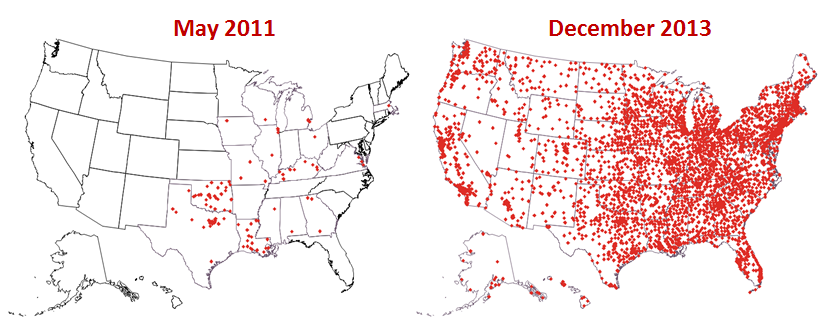
\includegraphics[scale=.6]{graphics/QS-Hospitals-Receiving-Payments-for-MU-and-Adoption.png}
    \caption*{Source: HealthIT.gov}
    \label{fig:meanuse}
\end{figure}

On a daily basis, a physician spends approximately 23.7\%, 17\%, and 15.5\% of their time on documentation, chart review, and inbox management, respectively which are the most time consuming portions of EHR use (\cite{arndt2017tethered}). In all, if a physician works for 12 hours, they spend roughly 3.2 hours with patients and 5.9 hours interfacing with an EHR, an example of which is shown in Figure \ref{fig:EPIC}. Despite a large amount of time spent with them, physicians still continue to report frustration over EHR use. The most time consuming functions are also reported as the most frustrating (\cite{dymek2021building}). A physician still likely spends almost 2 hours a day managing their inbox: deleting duplicate messages, sifting through messages meant for other members of a care team, and searching relevant information (\cite{dymek2021building}). Another common issue physicians face is the lack of usability of EHR systems, that functions either take minutes to locate or load. Hospitals often provide training upon adoption, but rapid system upgrades and changes make familiarity with the system difficult. 

\begin{figure}[ht]
    \centering
    \captionsetup{width=.4\linewidth}
    \caption{Screenshot of EHR System}
    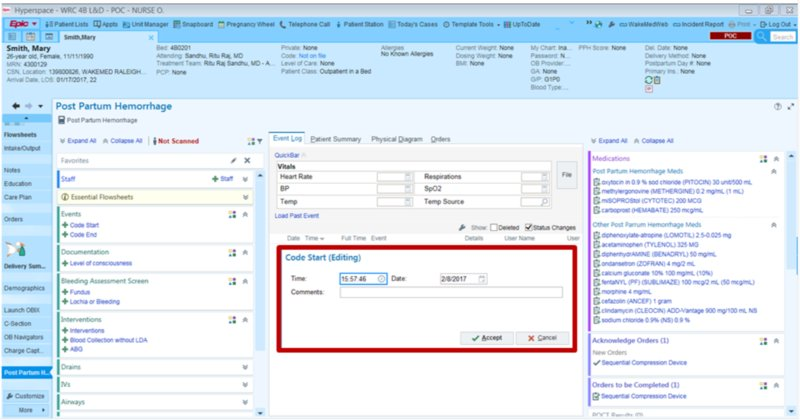
\includegraphics[scale=.4]{graphics/epic-ehr-screenshot.jpg}
    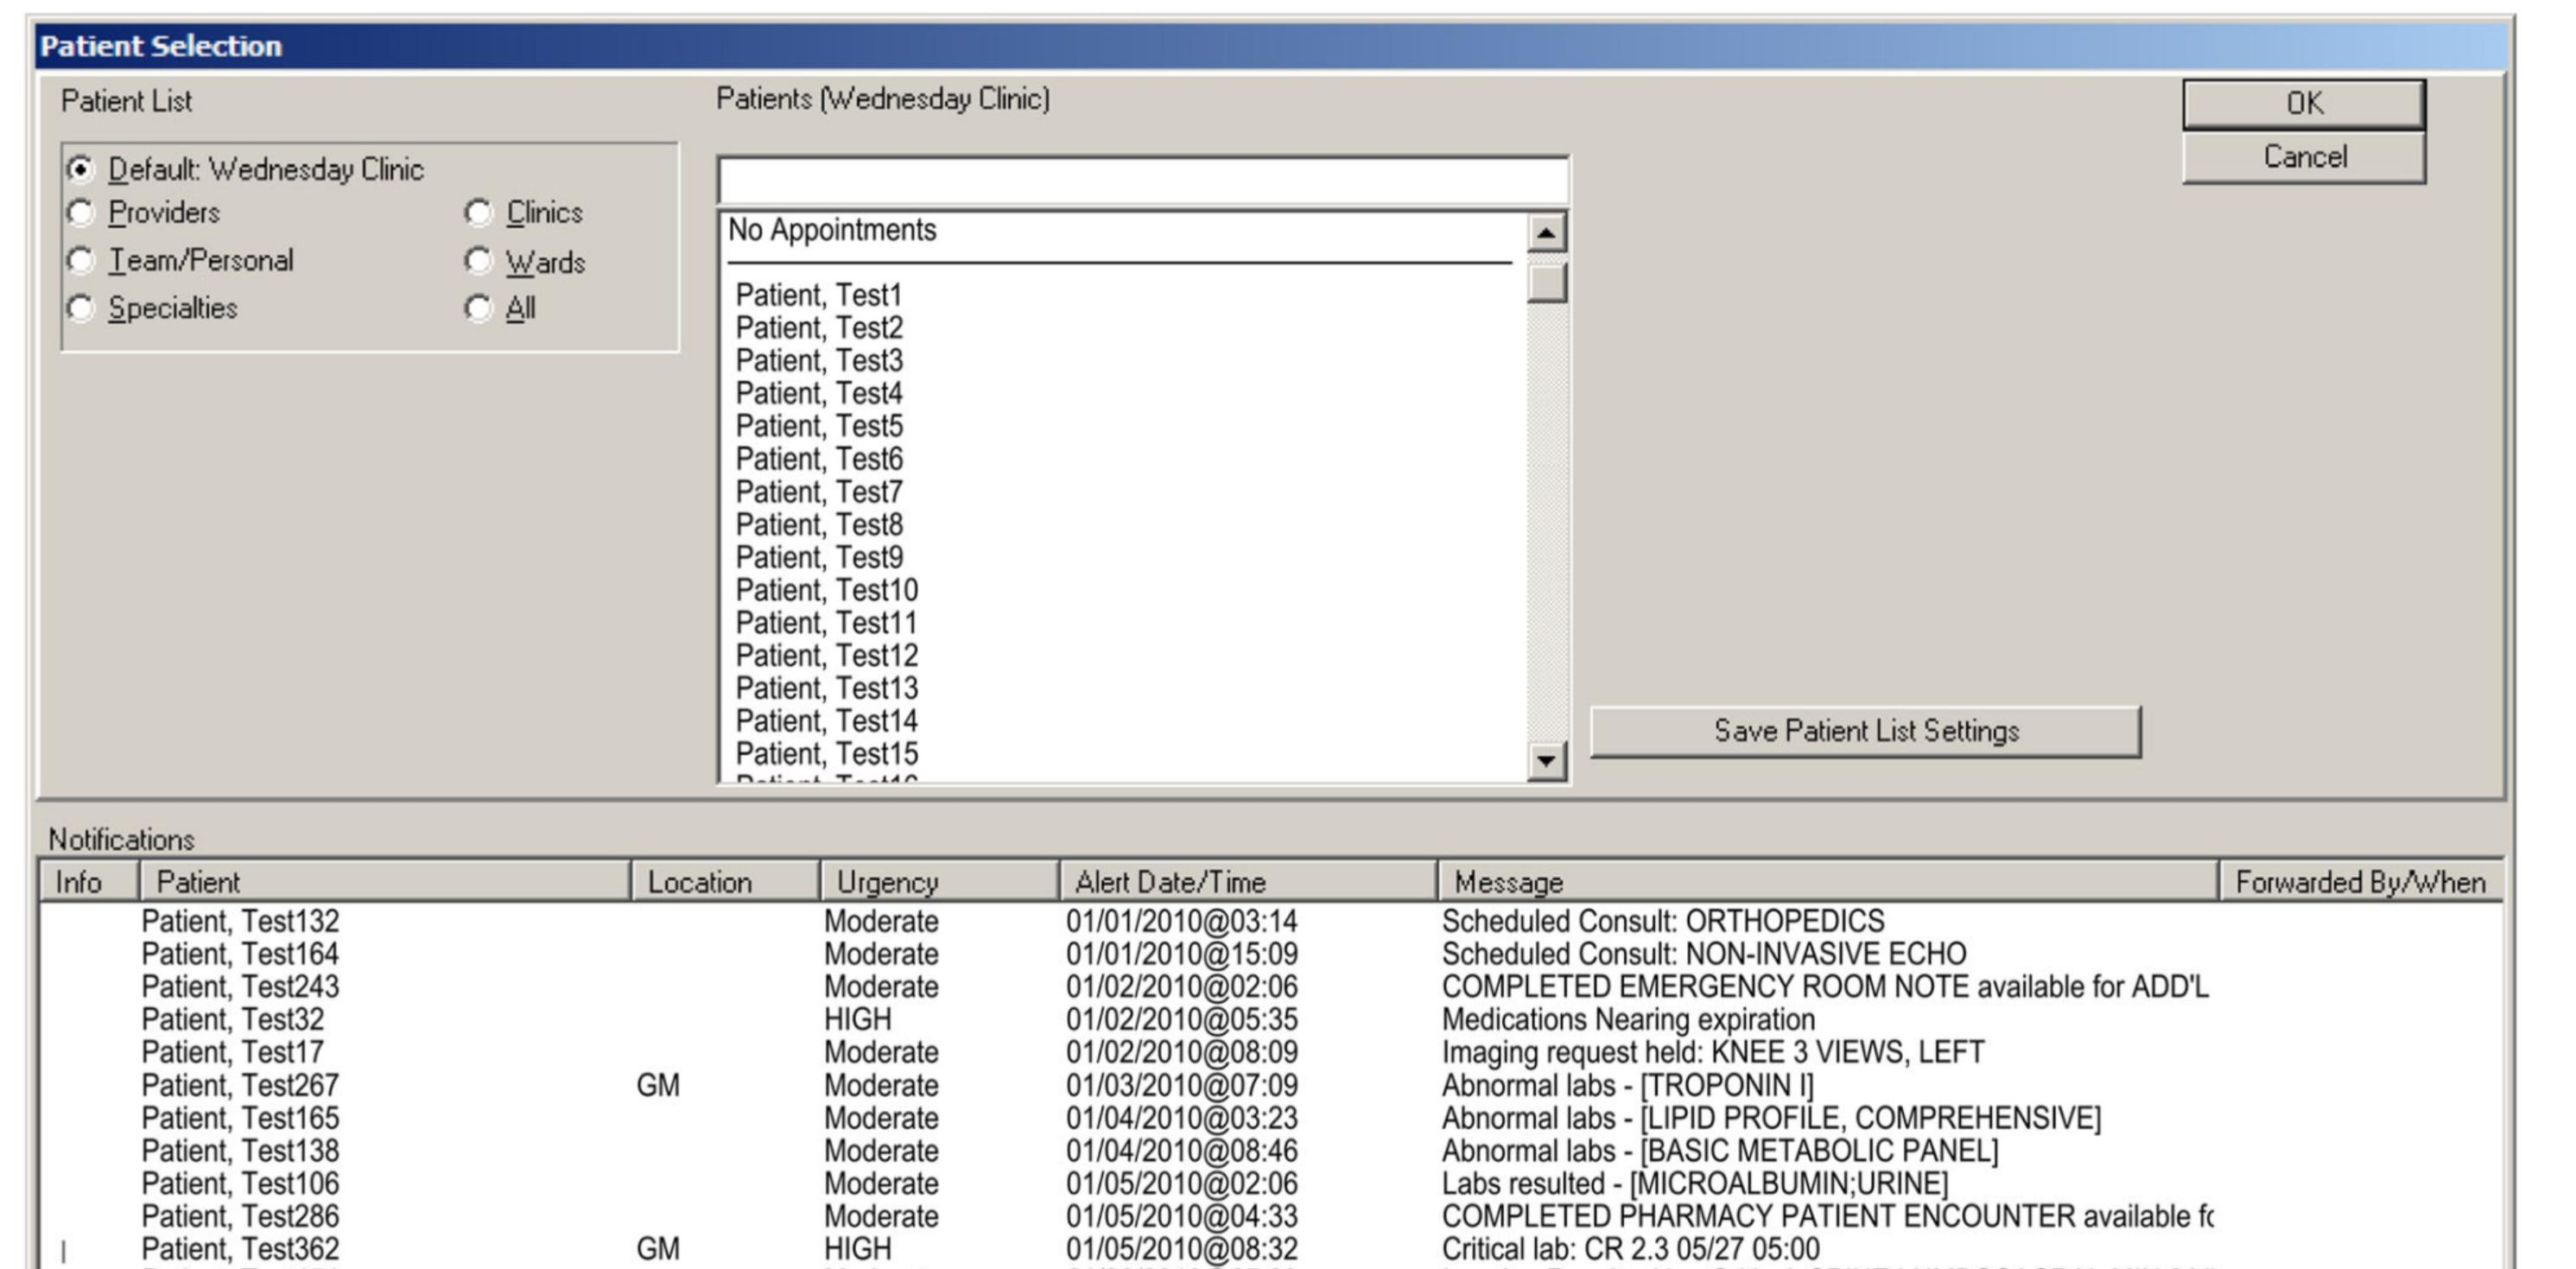
\includegraphics[scale=.11]{graphics/EHRimage2.jpg}
    \label{fig:EPIC}
\end{figure}


\subsection{EHR and Physician Labor Markets}

This section serves to outline the potential responses of hospitalists to EHRs based on their incentives. The physician behaviors that I consider in this analysis are closely related and should not be taken as independent. For example, a physician's choice of work setting depends on their decision to prolong retirement, and billing activity depends on work setting. Thus, I discuss the behaviors in stages of decision making. 

\subsubsection{Retirement}

Workers in developed countries tend to plan for formal retirement well in advance. Generally, an exogenous shock to a worker's environment is not expected to change retirement age due to the amount of planning necessary to formally leave the labor force. Classic retirement models structure the decision of retirement by maximizing expected lifetime utility based on future earnings and retirement benefits, or choosing to prolong retirement only if the expected earnings gain from doing so is positive (\cite{gustman1986disaggregated}, \cite{stock1990pension}). However, physicians typically make this decision differently than workers in other industries. Most physicians plan to retire at age 60, but do not actually retire until age 69 (\cite{collier2017challenges}). When the time to retire comes, many physicians hesitate to abandon patients they have seen over the course of their career. The decision to delay retirement is not financial, but altruistic. Thus, retiring may be in a physician's choice set years before the realized decision to leave the labor force. 

It is important to note that age is the most important factor in the decision to retire, implying that a 35 year old physician has very different incentives than a 65 year old physician, and a technology shock will affect the age groups differently. First, I consider physicians already of retirement age ($>=60$) when a new technology is implemented. While payment schemes, wealth, and retirement benefits certainly impact retirement since, on average, those in this age group have already prepared financially to retire. Then, a physician will only retire if the utility from working is less than the utility from retiring, where utility depends on job satisfaction and personal life factors. Exogenous EHR implementation affects the decision to retire through job satisfaction. If EHRs impose a burden on daily tasks, there is an inverse relationship between EHR exposure and utility from continuing to work. If EHRs make daily tasks easier, there is a positive relationship. Thus, for a physician indifferent between retiring and continuing to work, EHRs induce retirement if they impose a cost in terms of job satisfaction, or induce continued working life if they impose a benefit to job satisfaction. Media articles focusing on interviews with physicians suggest that the implementation of EHRs did in fact lead to retirement in older physicians (\cite{ringel_2019}, \cite{loria_2020}). 

Formal retirement (leaving the labor force altogether) is not the only way for physicians to transition out of a clinical role. There are opportunities for physicians of any age to switch careers towards administrative roles, teaching, consulting, or hospital management. While it is unlikely that early career physicians are formally retiring, physicians of any age could be career switching. This decision is impacted similarly to the above discussion regarding formal retirement, where a physician who is indifferent between clinical work and career switching can be affected one way or the other based on how an EHR impacts job satisfaction. As I discuss in Section \ref{sec:data}, I only observe whether a physician stops seeing Medicare patients, not whether they retire or career switch. Thus, the term retirement for the purpose of this paper indicates no longer seeing patients, and makes no assertion about what the physician does afterwards. A physician is said to retire in a given year only if it is the first year in which the physician has no future Medicare claims.



\subsubsection{Work Setting}

For most physicians, EHRs will not impose a large enough cost (or benefit) to change the duration of working in clinical settings. However, there are other ways physicians might change their behavior under drastic changes to their current working environment. For those who remain practicing, changing the physical place of work may allow the physician more control over which technologies they use. Some hospitalists work under contract full time for one medical practice, where they have a consistent shift schedule, while others contract themselves out to multiple hospitals, offices, or both. While I do not have sufficient data to observe the type of hospitalist each physician is, I investigate the incentives faced by each type.

First, I consider those who are in a relatively binding contract with the hospital. For hospitalists under full time contract with a medical practice, the physician is more tethered to the hospital. This could impact the response to EHR implementation in that hospital in two ways: (1) through potentially increased use of the EHR in its initial phases, and (2) limited access to other work settings. A typical contract requires 90 to 120 days termination notice and some contracts include do not compete clauses (\cite{yasgur_by_-_yasgur_2016}), making a shift in work setting costly or excluding it from the choice set. Since these hospitalists are established in their hospital, they work a significant amount of time there. When an EHR is implemented, they may become familiar with it more quickly and be less likely to desire to switch work settings. Thus, I classify these physicians as ``sticky", since they are not able to change behavior in the short run.

Alternatively, there may be hospitalists that work in multiple hospitals or work in both hospitals and offices throughout the sample period. If one hospital implements a costly (or beneficial) EHR, these workers can more easily shift all or some of their work towards (or away from) different facilities to allocate to the place where they gain the most job satisfaction. As this type of hospitalist is less sticky, if there is any effect of EHR exposure on work setting it would be among this type. 


\subsubsection{Productivity}

There are still physicians who are not induced to change their behavior on the basis of retirement or work setting due to EHR implementation. A lack of response could be due to 4 factors: the hospitalist is bound to their current work environment, EHRs make no impact on the work environment, EHRs are costly, but not costly enough to shift, or EHRs improve job satisfaction in the current work environment. For physicians who make no physical changes to work environment after EHR exposure, it is natural to assess whether EHRs affect productivity, as a main purpose of the HITECH Act was to improve efficiency of care, specifically to decrease time spent on administrative burden. 

Whether EHRs affect productivity in terms of patients seen is theoretically ambiguous. If they serve their purpose to decrease administrative burden, the physician would be freed up to see more patients. In this case, productivity would increase. However, if utilizing an EHR actually imposes an additional administrative burden as suggested in physician interviews, the number of patients could either decrease or stay the same, indicating a decrease in productivity. Further, there is a unique relationship between EHR use and efficiency in terms of billing activity done by the physician. Billing activity refers to the number of claims filed per patient seen. EHRs may improve efficiency if they remove the need for repeated or excess testing. However, if having an EHR makes it easy for a physician to claim for additional items with the click of a button, the adverse incentive may lead physicians to claim for more items per patient.




\section{Data}\label{sec:data}

I construct a physician-level panel spanning from 2009-2017 which measures physicians' exposure to EHRs over time, labormarket outcomes, and other relevant physician, hospital, and practice characteristics. I describe the different data sets used to construct the panel below, and I include a detailed outline of data and variable construction in Appendix \ref{app:data}.

\subsection{Sample Construction}

The Medicare Data on Provider Practice and Specialty (MD-PPAS) is a database of physicians which details claim counts, physician specialty, and practice location from 2009-2017. Variables included are physician NPI, primary and secondary specialties, patient count and total billing counts, and fraction of patients seen in different settings. I only include physicians who reported their primary specialty as hospitalist (physician who self-identifies as hospitalist or has 90\% of patients in inpatient setting), internal medicine, general practice or family practice in at least one year. Since the focus of the analysis is physicians working in hospitals, I also drop physicians with less than 70\% of patients in a hospital setting in all years, and I drop physicians with insufficient claim counts to show indications of behavior. I use this data to construct the dependent variables for my analysis. Generally, these include the decision to retire (leave clinical work), switch to a different work setting, number of patients seen, and overall billing activity. I describe these outcome variables and their construction in detail in Section \ref{sec:outcome}.


CMS Shared Patient data records annual information on frequency of billing associated with the same patient across providers within a given time period. These data are available from 2009 to 2015. For example, if a primary care physician refers a patient to a specialist, then those two physicians have that particular shared patient in common. The number of shared patients are collected in 30, 90, or 180 day intervals. I focus on the 30 day interval, and I employ this data to detect physicians who work closely with hospitals. I limit the entities by tax-code to only include shared patients for physician-hospital pairs, where the physicians in these pairs match the physicians from MD-PPAS. The types of physicians are already limited to primary care, but there still may be office-based primary care physicians in the shared patient data. Therefore, I limit the sample of pairs based on a threshold of same day patients which depends on the number of years the physician appears in the data. I only include physician-hospital pairs who have non-missing data with at least 30 shared patients per year.


Using hospital National Provider Identifier (NPI), I link the physician-hospital pairs from the Shared Patient data to the American Hospital Association (AHA) survey, which contains information on hospital-level EHR use and other characteristics. I record the first year a physician is exposed to an EHR based on implementation in the hospitals they share patients with. A hospital can answer the question of whether they use an EHR with either ``Partially", ``Fully", or ``Not at all". Since partial implementation of an EHR does not guarantee sufficient use, I define a hospital as implementing an EHR the first year they answer ``Fully". I then aggregate this data to the physician level. Since the Shared Patient data does not extend to 2017 as the MD-PPAS data does, in the analysis I drop physicians who are not treated by 2015, as I do not observe whether they become treated in 2016 or 2017. That is, the data contains no units which are ``never-treated".

Finally, I include a physician's graduation year from Physician Compare. I limit to physicians who graduated before 2005, as anyone who graduated medical school after that will be finishing residency during the span of the data and will exhibit labor market changing behavior which could be correlated to EHR exposure purely because of switching work settings during a time of rapid EHR implementation.There are various thresholds used in the construction of this final data, including how many shared patients constitutes a physician-hospital relationship. The details of such thresholds are explained in Appendix \ref{app:data}. To ensure that my results  are not sensitive to various levels of the thresholds, I estimate the effect of EHR exposure on all outcomes under different combinations of data limitations. The specification charts with these results are shown in Appendix \ref{sec:chart}, and I discuss each in conjunction with the main results. 

\subsection{Outcome Variables}\label{sec:outcome}

The first dependent variable I consider is the decision for a physician to stop seeing Medicare patients, which I refer to as retirement. This variable is constructed as follows: 
$$\text{retire}_{it}=\mathbbm{1}\{FC_{it}=0 \text{ and retire}_{i,t-1}=0\}, $$
where $FC_{it}=\sum\limits_{j=t+1}^T\text{(claim count)}_{ij}$ is all future claims for physician $i$ in year $t$. Retire is therefore an indicator variable set to one in the first year that a physician has no claim counts at any point in the future. \footnote{Alternatively, I could also define retirement using future number of patients. I use claim count for a more conservative measure of retirement, but using patient count yields identical results. In Appendix \ref{sec:changes}, I limit the sample years to 2009-2015 to assess the robustness of the main retirement definition.}

Next, I consider whether physicians exhibit behavior that suggests they have shifted setting or location of work. I consider the fraction of patients a physician sees in an office-based setting, which is directly available in the data. Then, I construct an indicator variable equal to one if a physician sees any number of patients in an office-based setting, which offers less variation but captures the extensive margin of working in an office. Finally, I consider outcome variables which explore productivity and efficiency, the number of patients seen and claims filed per patient.


\subsection{Summary Statistics}

I show summary statistics of relevant variables for the entire sample in Table \ref{tab:sumstats}. Only 3\% of physicians (approximately 770) retire over the course of the panel. 30\% of the physician-year observations indicate working in an office in some capacity, with about a tenth of the number of patients being seen in an office setting. By construction, all physicians are exposed to an EHR at some point in the sample, so the variation in treatment variables comes from the timing of exposure. Physicians are typically exposed about one fourth of the way through the sample, but there is a positive number of physicians first exposed in each year from 2009-2015. The average physician is 45 years old and works with 1.5 hospitals and 1.3 systems. 
\import{Table Code}{overall stats.tex}


I also include a table of means comparing physicians below and above retirement age in Table \ref{tab:splitstats}. Senior physicians see more patients and work in more hospitals on average than younger physicians. They also see a larger fraction of patients in an office setting and are more likely to work in an office in general. The age groups are exposed to EHRs similarly.

\import{Table Code}{split stats.tex}


In Figure \ref{fig:treatmentgraph}, I present a graph of the variation in treatment over time. In 2009, 28\% of the sample of physicians were already exposed to an EHR. That is, three quarters of the sample had no affiliation with EHRs at the beginning of the sample period. Since I drop any physicians who do not have exposure to an EHR by 2015, 100\% of the sample is exposed by the end of the sample period. The darker line shows the underlying variation in this variable, hospitals implementing EHRs over time. 

\begin{figure}[t]
\centering
\captionsetup{width=.45\linewidth}
    \caption{Treatment Variables Over Time}
    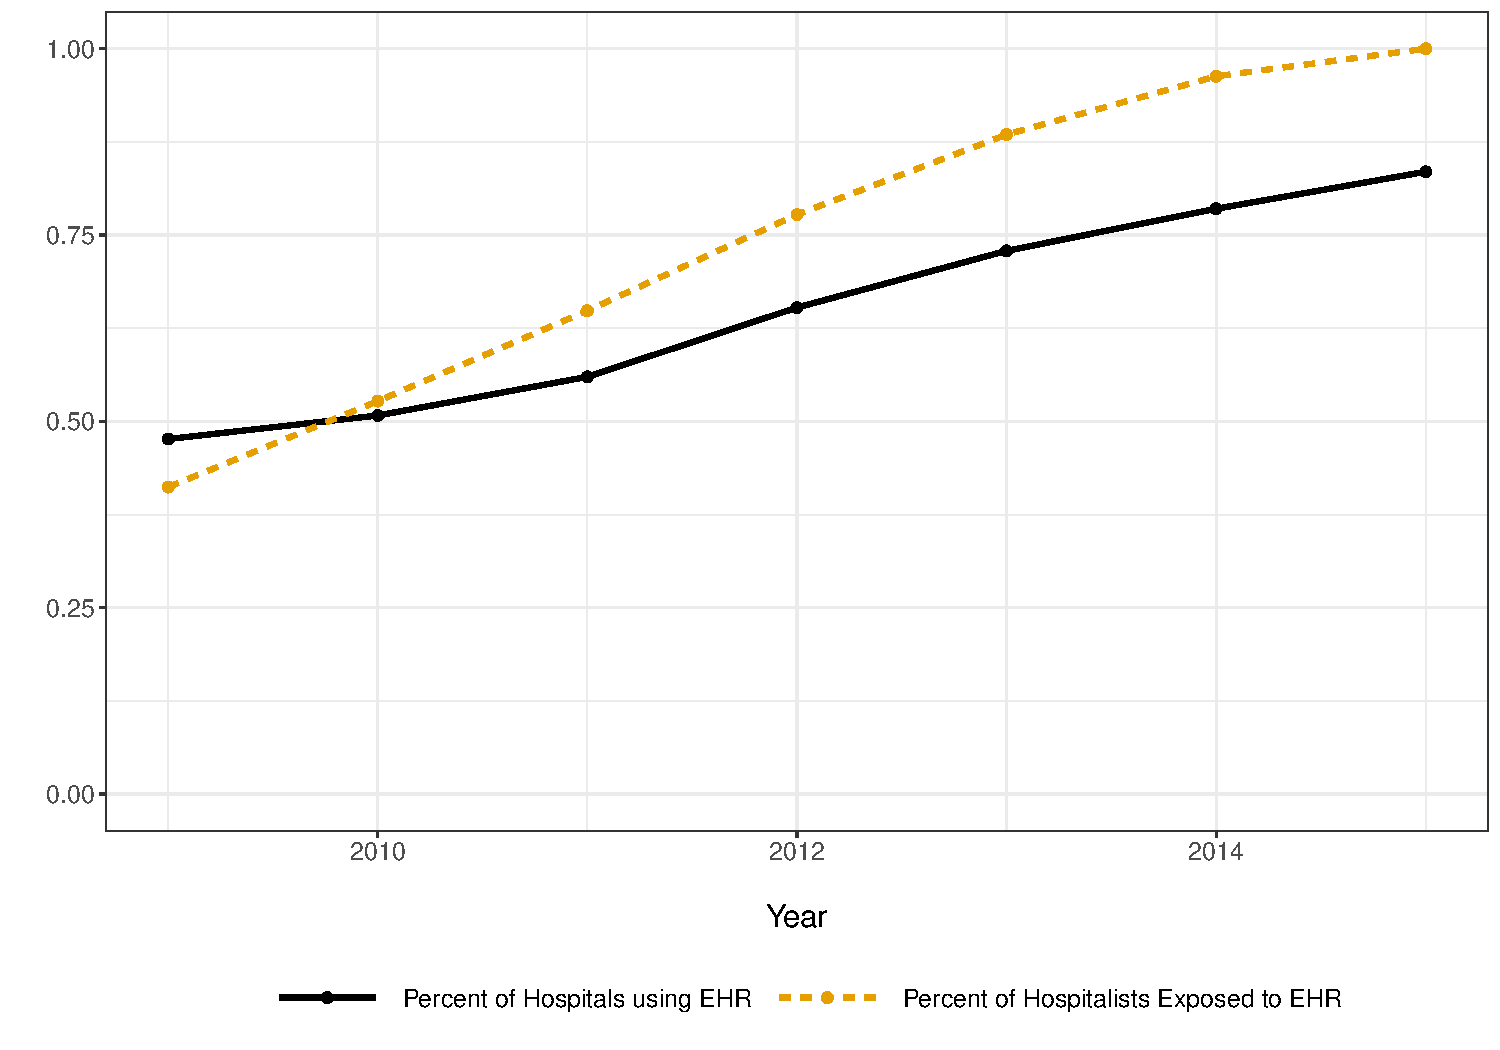
\includegraphics[scale=.5]{Objects/sum_stats_year.pdf}
    \label{fig:treatmentgraph}
\end{figure}



\section{Empirical Strategy}\label{sec:empstrat}

I treat EHR implementation as an exogenous treatment variable, and I estimate average treatment effects of EHR exposure on the outcomes discussed. In this setting, treatment effects are heterogeneous across physicians who are exposed in different years since the underlying characteristics of hospitals who adopt in different years may be correlated with the decision to adopt. Therefore, to avoid negative weighting issues this causes in a classical two way fixed effects event study specification, I instead estimate average treatment effects for a specific group $g$ at time $t$: 
$$ATT(g,t)=\mathbbm{E}[Y_t(g)-Y_t(0)|G_g=1],$$
where $G_g=1$ for those in group $g$. A group indicates all physicians treated, or first exposed to an EHR, in the same year. To estimate the heterogeneous treatment effects, I employ the doubly robust estimator established in \citeauthor{sant2020doubly} (\citeyear{sant2020doubly}). Other estimators that similarly address the concerns yield similar results, presented in Appendix \ref{app:estimators}. I also present classical two way fixed effects results with physician and year fixed effects in Appendix \ref{app:estimators}.

I aggregate the group time estimates over groups to a more familiar event study plot. For select outcomes, I present the original pre-aggregation estimates to show that results are not driven by a particular year of treatment.  Further, a weighted average of estimates is taken to provide a single $ATT$ value for each outcome; these values are presented in the notes of each results plot. Simultaneous confidence bands, calculated using bootstrapped standard errors, are also presented. 

\subsection{Identification Assumptions}

There are several assumptions necessary to identify the parameters of interest, $ATT(g,t)$. First, I assume that treatment is not reversed. That is, once a physician is exposed to an EHR, they cannot be un-exposed. For physicians that do not switch hospitals, this assumption is supported by both the institutional details of hospital EHR implementation and the data itself. An EHR is a costly technology and requires a significant amount of collaboration to implement. A hospital does not have incentive to un-implement an EHR once it is implemented. They may add features or switch vendors, but do not reverse EHR use. This institutional detail is supported by Figure \ref{fig:hosp_treat}, which shows EHR status of a 2\% random sample of hospitals over time.\footnote{Note that out of the 81 hospitals included in the random sample, 4 of them show a reversal of treatment status. Upon further inspection, each of these hospitals show such a reversal due to a discrepancy in the coding of whether the hospital uses an EHR partially or fully. Those who use the EHR partially are coded as not fully implementing an EHR since it is not clear whether physicians in the sample would be exposed yet or not. Hospitals with this discretion are coded as implementing an EHR in the first year that they answered "fully" to the survey question.} When considering the outcomes of patient count and billing activity, it could be that a physician moves from a hospital that uses an EHR to a hospital that does not, affecting the number of claims observed in the data. Thus, I limit the sample of physicians for these outcomes to those who remain with the same set of hospitals throughout the entire period. I discuss this limitation to the data further in Section \ref{sec:patientcount}.

\begin{figure}[ht!]
    \centering
    \captionsetup{width=.7\linewidth}
    \caption{Hospital EHR Adoption Over Time}
    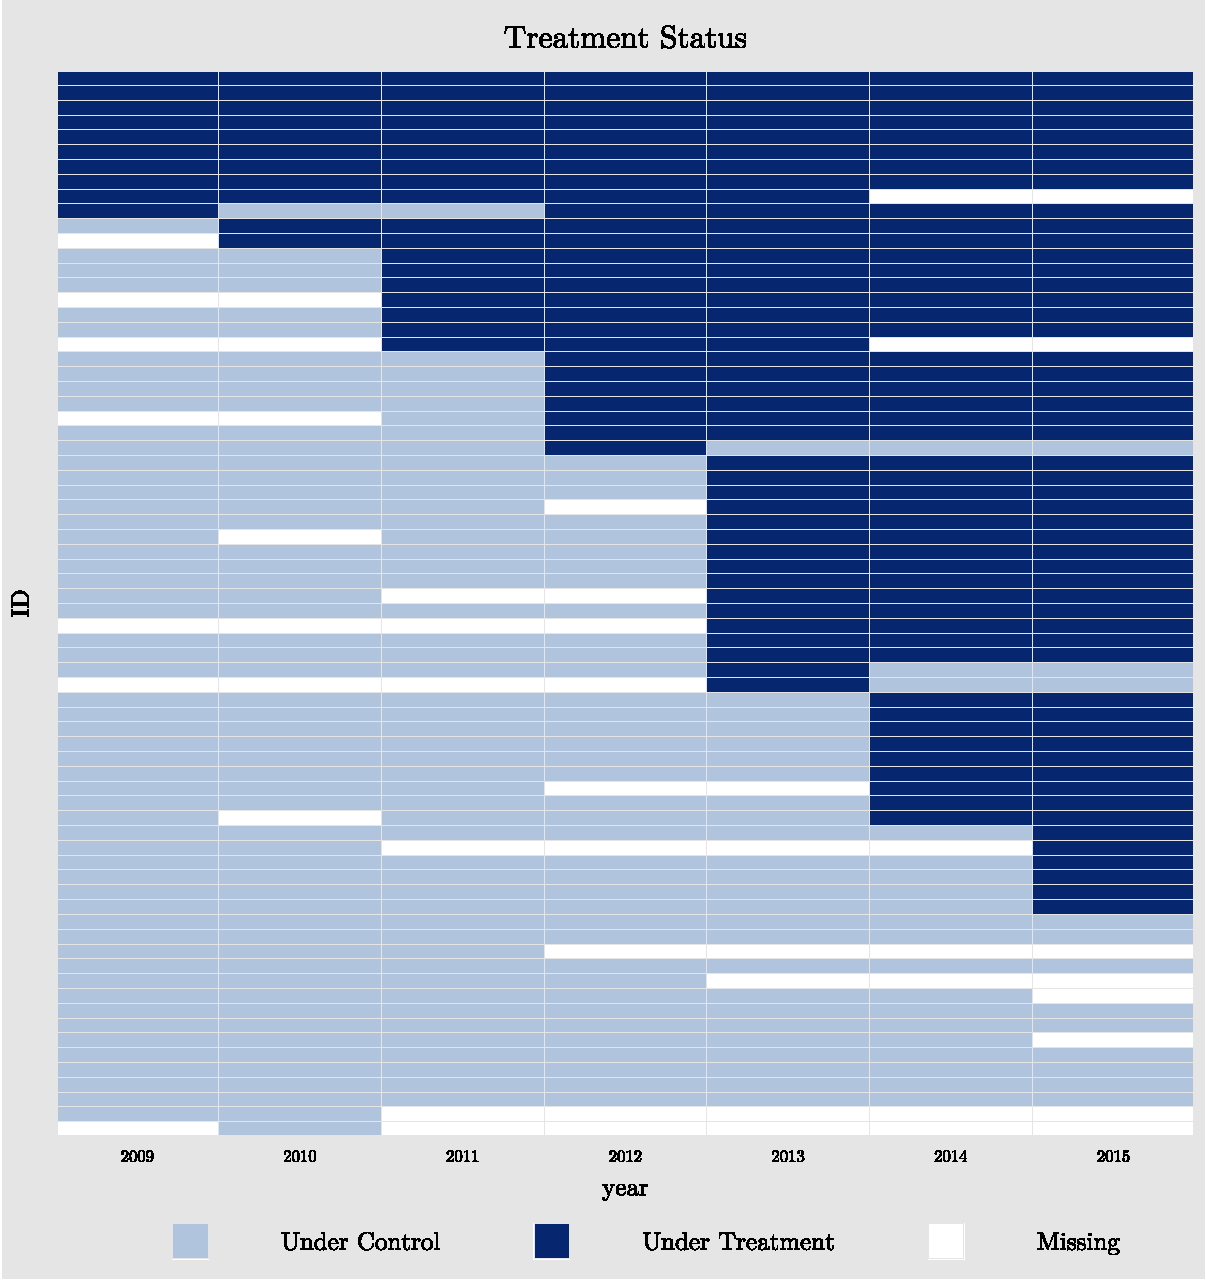
\includegraphics[scale=.5]{Objects/hosp_treat.pdf}
    \label{fig:hosp_treat}
\end{figure}

Second, I assume physicians do not anticipate EHR exposure prior to occurrence. This may be a concern if physicians learn that the system will be implemented and change their behavior beforhand. Generally, even a complex EHR system can be completely set up within a year, and most systems take 6 to 9 months (\cite{uzialko_2021}). Therefore, I proceed in the main specification assuming no anticipation. However, I explore and present results for a one year anticipation period in the specification charts in Appendix \ref{sec:changes}, and I find that accounting for one year of anticipation does not drastically change my findings.  

As is usual in a difference-in-differences framework, I assume a version of parallel trends based on not-yet-treated units. I assume that, conditional on years of experience, average outcomes for those treated in group $g$ would have followed a parallel trend as those in groups treated in later periods. This assumption would be violated under external conditions in certain years that may be correlated with labor markets, such as a major recession. The time period I study, 2009-2017, is reassuringly stable. In my analysis, I present p-values for a Wald test of pre-trends. Further, I investigate pre-trends extensively in Appendix \ref{sec:pretrends} by allowing for specified violations in the parallel trends assumption (\cite{rambachan2019honest}). I find that most outcomes are very robust to violations in the parallel trends assumption. 

To interpret these estimators as the causal effect of EHR exposure on various labor market outcomes, there are additional institutional assumptions necessary. First, I assume that when a physician works in an electronic record utilizing-hospital, they utilize the electronic health record system fully. That is, there are no ways for the physician to continue practicing without using the EHR. I investigate this assumption in Section \ref{sec:dataass}. While physicians may create work-arounds to ease the burden of EHR use, it is inevitable that they will need to interact with the technology in some capacity. Second, I assume that a physician's exposure to EHRs is exogenous. That is, the physician does not influence the hospital's decision to implement an EHR. I investigate this assumption in Section \ref{sec:endogeneity}. 







\section{Effect of EHR Exposure on Labor Market Outcomes}


\subsection{Retirement}\label{sec:retire}


I present aggregated group time treatment effects of being exposed to an EHR on the likelihood of retirement for the full sample of physicians, as well as split samples for those at least 60 (typical retirement age) and less than 60 years of age in Figure \ref{fig:retirefirst}.\footnote{Alternatively, one could estimate the effect for more age groups and observe the relationship between the overall ATT and age. However, the data is not ideal for more than two age groups since the sample sizes decrease dramatically for certain groups.} These effects are a weighted average of the $ATT(g,t)$ parameters discussed in Section \ref{sec:empstrat}. Being exposed to an EHR leads to a .002 ppt increase in the likelihood of retiring in the first year after exposure, and a .005 ppt increase in the second year after exposure. While numerically small, these effects are statistically and economically meaningful relative to the proportion of physicians who retire in the sample, .03. That is, the effect represents a 7\% (16\% in the second year) increase in the likelihood of retirement relative to the mean. 

Even though there is no visual indication of a violation of the parallel trends assumption in the pre-periods, the p-value of a Wald test for pre-trends indicates some evidence for such a violation. In Appendix \ref{sec:pretrends}, I present confidence intervals robust to various specifications of a violation in parallel trends. Due to the rarity of retirement in the sample, the estimate becomes null with any specified variation in the parallel trend assumption. Since the pre-trend does not look strong in the first place, this is not too concerning. I present estimates for the overall $ATT$ under various specifications of the data in Appendix \ref{sec:chart}. The estimate found here falls in the upper range of estimates. All estimates are positive, yet some have confidence intervals that include zero. Closer examination into these estimates reveals that stricter thresholds on the data yield many of the null results. Even with additional noise in the estimates, the average of the upper and lower confidence intervals still indicates a positive effect of EHR exposure of retirement. Thus, the main finding is robust to various specifications.   

\begin{figure}[ht!]
    \centering
    \captionsetup{width=.85\linewidth}
    \caption{Effect of EHR Exposure on Retirement}
    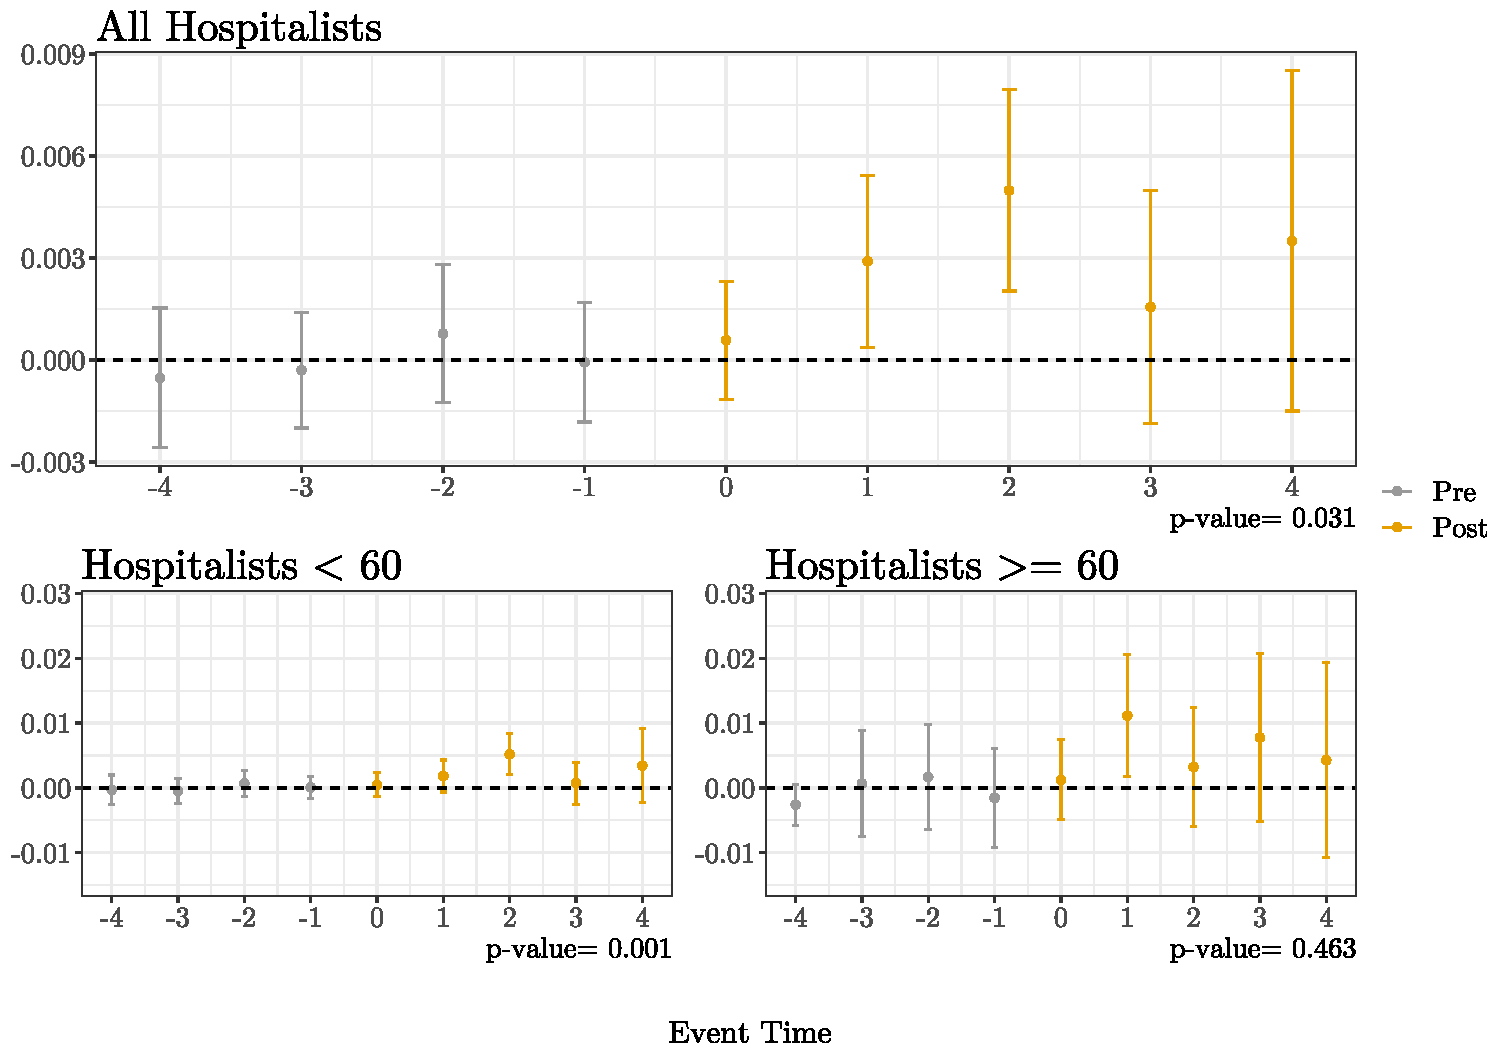
\includegraphics[scale=.6]{Objects/retire_plot.pdf}
    \label{fig:retirefirst}
    \vspace{2mm}
    \caption*{\footnotesize{\textit{Notes:} The top panel shows average group time treatment effects aggregated over groups to an event study plot. The bottom show these results for different subgroups of physicians by age. The p-value listed for each graph corresponds to a Wald test for pre-trends. Confidence intervals shown are simultaneous confidence bands accounting for multiple hypothesis testing. Overall ATT for all, $<$ 60, $>=$ 60 with SE in parentheses: 0.003 (0.0009), 0.002 (0.001), 0.006 (0.003), respectively.}}
\end{figure}


Next, I examine how the results differ when considering physicians in different age brackets: pre-retirement ($<= 60$) and typical retirement age ($> 60$). Interestingly, senior physicians are driving the positive estimate in the year after exposure, while younger physicians are driving the result for the second year after exposure. A retirement age physician is .01 ppts more likely to retire after being exposed to an EHR, a 25\% increase relative to the mean. In comparison, physicians less than 60 are not more likely to retire in the first year after exposure, but are approximately 16\% more likely to retire two years after exposure. There are two potential reasons for the different response time that relate to formal retirement vs. career switching. First, if younger physicians are leaving clinical work for administrative or consulting roles, the preparation time for this type of switch (preparing a resume, applying for new jobs, etc.) could be longer than one year, whereas formal retirement can be decided and executed within one year. Similarly, younger physicians may attempt to learn complex EHRs for a longer period of time before deciding the cost is too high. 

A potential concern is that physicians are not leaving a clinical setting, but only see patients with private insurance. While EHR use should not be directly correlated with Medicare patients, there may be an unobserved event leading physicians to stop seeing Medicare patients that aligns with EHR implementation. CMS publishes a list of physicians who have officially opted out of seeing Medicare patients and none of the physicians in my sample have selected into this option. Additionally, hospitalists do not have complete control over their composition of patients.  


\subsection{Place of Work}

I investigate another dimension by which physicians could change behavior: the extent to which they work in an office and whether this changes due to EHR exposure. The outcomes I consider are (1) an indicator variable equal to 1 if the physician has any positive number of patients in an office in a given year, shown in Figure \ref{fig:officefirst}, and (2) the fraction of patients a physician sees in an office in a given year, shown in Figure \ref{fig:officesecond}. This analysis does not include individuals who retire at any point in the sample, as a zero could indicate dropping out of the data instead of working solely in a hospital. 

EHR exposure increases the likelihood of working in an office by at least .04 ppts in every year after being exposed, where the effect increases over time (up to .1 ppts four years after exposure). This estimate is equivalent to a 15-38\% increase relative to the average proportion of physicians who work in an office. That is, physicians working only in a hospital are more likely to start working in an office after being exposed to an EHR, and these effects are just as large as those on retirement. However, unlike the estimated retirement effects, the increased likelihood of working in an office is persistent over time, which suggests that EHRs impact work environment in hospitals for several years after implementation. 

I consider the robustness of these results to various violations in the parallel trends assumption in Appendix \ref{sec:pretrends}, where the findings are similar. Further, I compare this finding with various specifications to data thresholds and variable definitions with an estimate chart in Appendix \ref{sec:chart}. I find consistently positive and significant coefficients ranging from .02-.08 percentage points. Thus, the main finding is on the high end of the range of estimates. While all estimates are positive, some variations that drive the estimate down slightly are limiting years to 2009-2015, and using the low integration definition of EHR exposure. I discuss this further in Appendix \ref{sec:changes}, and confirm that my finding is robust to specification changes. 



\begin{figure}[ht]
    \centering
    \captionsetup{width=.85\linewidth}
    \caption{Effect of EHR Exposure on Likelihood of Working in Office}
    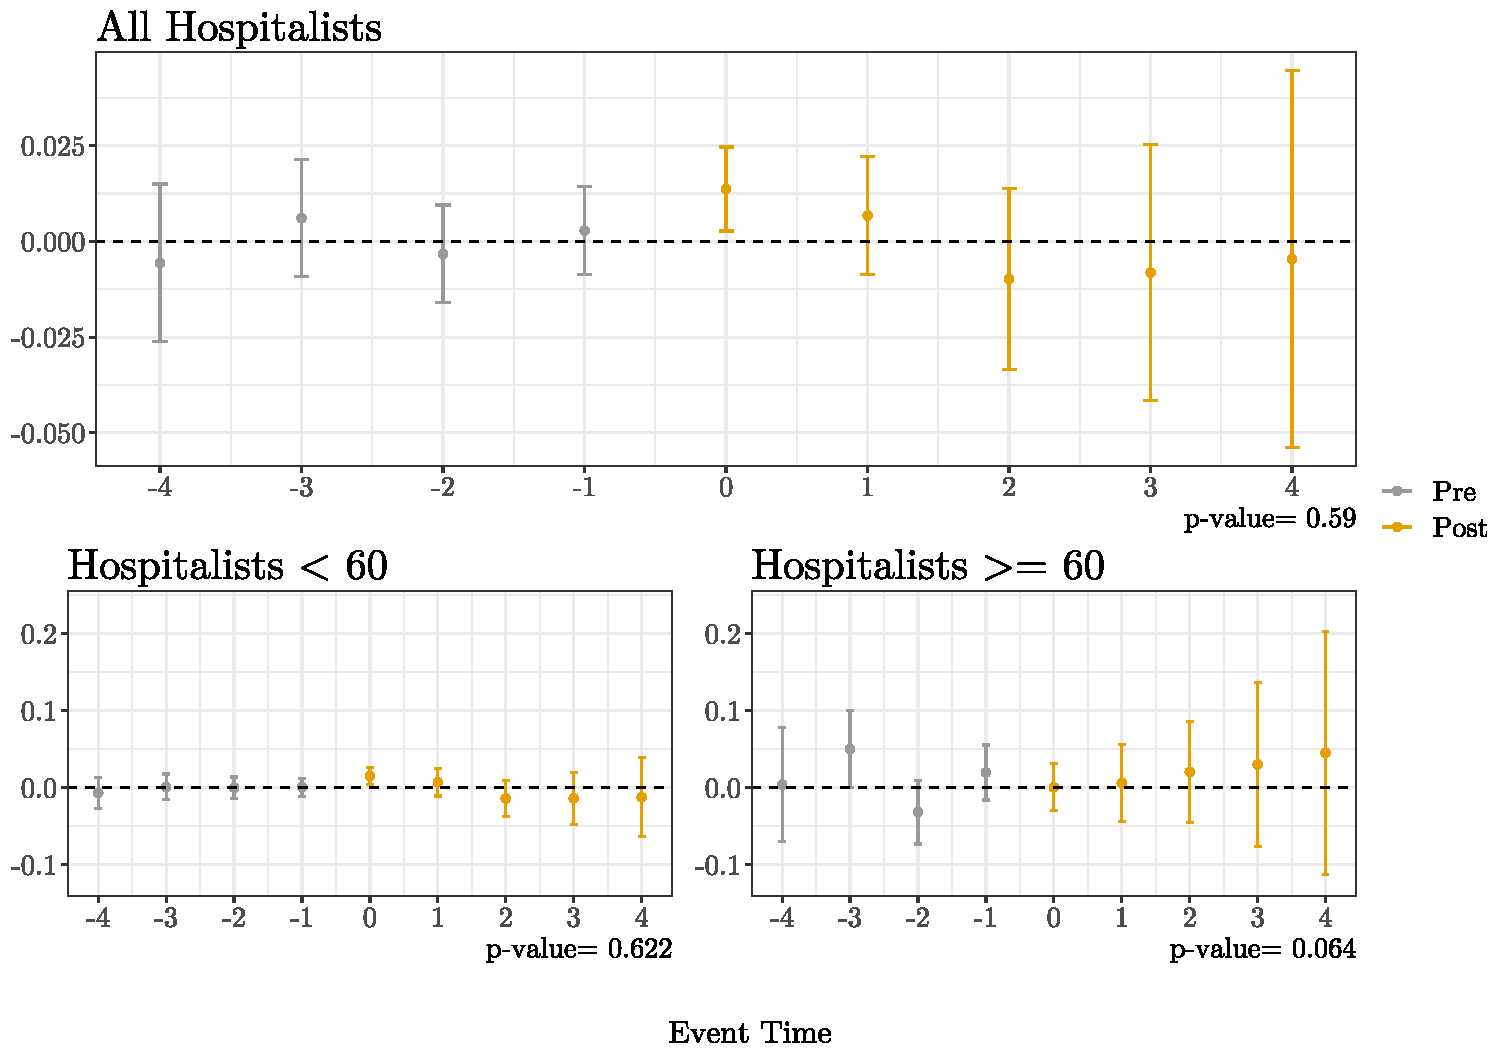
\includegraphics[scale=.6]{Objects/officeind_plot.pdf}
    \label{fig:officefirst}
    \vspace{2mm}
    \caption*{\footnotesize{\textit{Notes:} The top panel shows average group time treatment effects aggregated over groups to an event study plot. The bottom show these results for different subgroups of physicians by age. The p-value listed for each graph corresponds to a Wald test for pre-trends. Confidence intervals shown are simultaneous confidence bands accounting for multiple hypothesis testing. Overall ATT for all, $<$ 60, $>=$ 60 with SE in parentheses: .07 (0.008), .06 (0.008), 0.12 (0.03), respectively.}}
\end{figure}

To continue investigating how different ages may respond differently to technology, I also present estimates for physicians $<60$ and $>=60$ separately in the bottom panel of Figure \ref{fig:officefirst}. Unlike the choice to retire, the age groups are both responding to EHR implementation in all years after exposure. The magnitudes for senior physicians continue to increase over time, whereas the estimates for younger physicians level out. However, senior physicians are more likely to work in an office than younger physicians on average, so both groups exhibit similar increases relative to the mean. 

The previous results are driven by physicians who are not already working in an office prior to EHR exposure, but it could also be the case that physicians who already work in both settings before EHR exposure change the amount of work they do in an office. Thus, I estimate the effect of EHR exposure on the fraction of patients seen in office based settings.\footnote{Since this variable is tied to the total number of patients seen, I also estimate this analysis with the outcome of total number of patients seen in an office and the results are identical.} The estimates show an increase in the fraction of patients seen in office settings after the physician is exposed to an EHR. In the year of exposure, the fraction of patients increases by .06, and by the fourth year after exposure the fraction of patients increases by .12 due to exposure. Since the physicians included in the sample are meant to have close ties with hospitals, the average fraction of patients seen in an office is low, at .08. Thus, the observed effect I estimate here is massive as it is equivalent to a 75-150\% increase in the fraction of patients seen in an office relative to the mean. Further, the variation in this variable can either be driven by physicians who already worked in an office or those who did not and then began working in an office after exposure. When I partition the sample into prior office work, the effects are identical for both groups. 


\begin{figure}[ht]
    \centering
    \captionsetup{width=.85\linewidth}
    \caption{Effect of EHR Exposure on Fraction of Patients Seen in Office}
    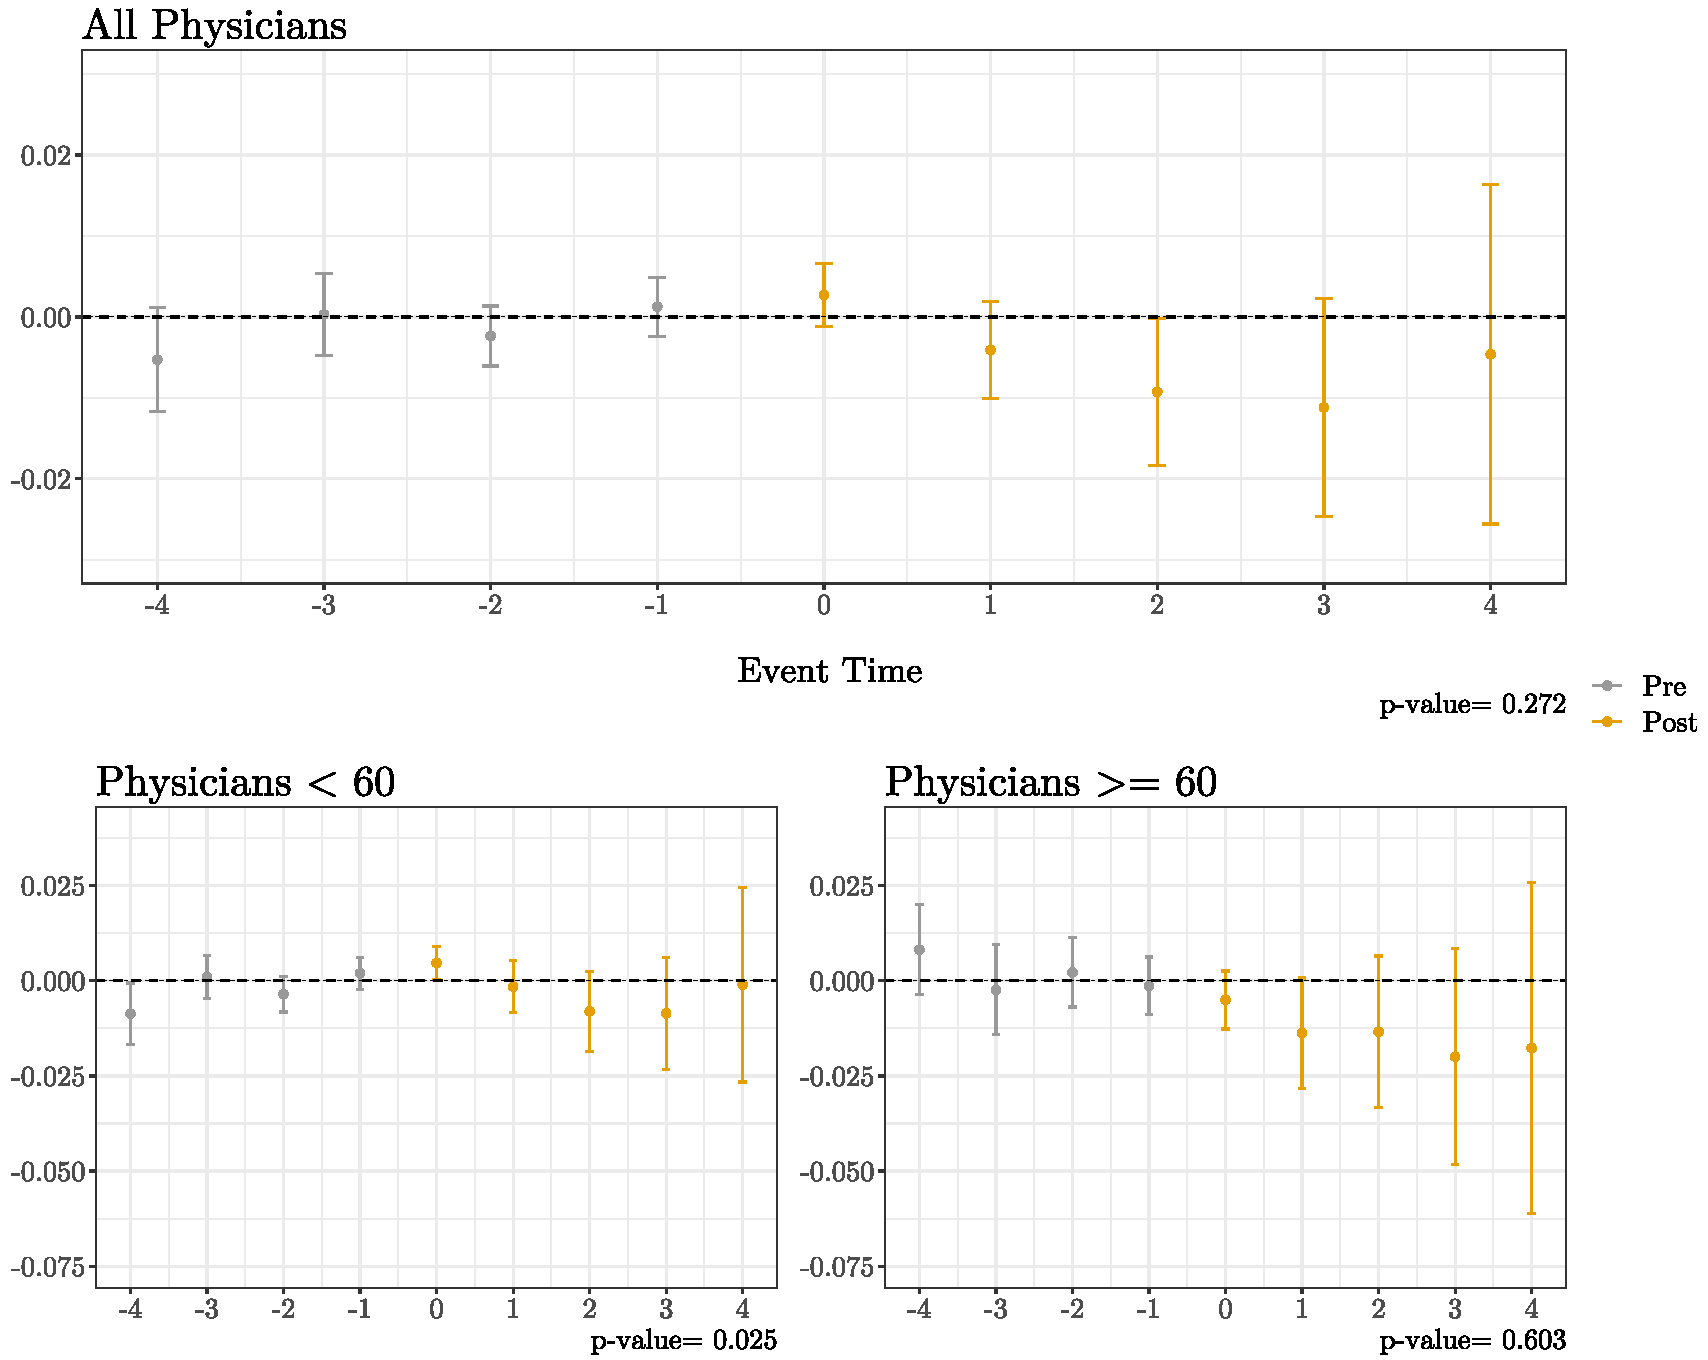
\includegraphics[scale=.6]{Objects/officefrac_plot.pdf}
    \label{fig:officesecond}
    \vspace{2mm}
    \caption*{\footnotesize{\textit{Notes:} The top panel shows average group time treatment effects aggregated over groups to an event study plot. The bottom show these results for different subgroups of physicians by age. The p-value listed for each graph corresponds to a Wald test for pre-trends. Confidence intervals shown are simultaneous confidence bands accounting for multiple hypothesis testing. Overall ATT for all, $<$ 60, $>=$ 60 with SE in parentheses: .08 (0.003), .07 (0.003), 0.13 (0.01), respectively.}}
\end{figure}

I also investigate pre-trends for this outcome in Appendix \ref{sec:pretrends}, where I find that under various assumptions of the form of violation in parallel trends, the estimate remains positive and significant of similar magnitude. Further, under different combinations of data specifications I find consistently positive and significant results, as shown in Appendix \ref{sec:changes}. However, the range of magnitudes is large: .01 to .1 percentage points. Thus, the main finding is large relative to these other estimates. Both accounting for anticipation and limiting sample years push the magnitude of the estimate down. Taking the average of these confidence intervals shows that the positive effect of EHR exposure on the fraction of patients seen in the office is robust to many combinations of data thresholds. 

The increasing trend over time remains the same for physicians of different age groups. However, senior physicians have larger estimated magnitudes in each year after exposure. Since senior physicians have more patients in an office on average, the percentage change is similar between the two age groups. 



\subsection{Patient Count and Billing Activity}\label{sec:patientcount}

As a measure of productivity/efficiency, I now estimate the effect of EHR exposure on patient count and billing activity per patient. If the sample includes physicians who shift place of work, this may lead to biased estimates since a physician could switch hospitals due to an EHR and then change practice behavior due to the change in environment, not due to the EHR. Thus, I limit to physicians who work with the same one hospital through the entire sample. These hospitalists do not retire or see patients in another hospital, implying that when an EHR is implemented, the physician remains utilizing the EHR for the remainder of the sample. 

The effect of EHR exposure on patient count is shown in Figure \ref{fig:patient}. For hospitalists of any age, patient count increases by 22.4 patients in the year of EHR exposure, 45.4 patients in the year after exposure, 28.1 patients in the second year after exposure, and approximately 20 in the third and fourth year after exposure. These estimates translate to a 6-14\% increase in the number of patients seen relative to the mean. Interestingly, when splitting the sample by age group, the effect decreases three and four years after exposure for younger physicians, while the effect for senior age physicians remains persistent over time, suggesting that technology's effect on productivity in the long run depends on worker type (in this case, age). 

Again, I present a sensitivity analysis considering the parallel trends assumption in Appendix \ref{sec:pretrends} and find that this increase in patient count is robust to violations in the parallel trends assumption. I also present estimates under different data specifications in Appendix \ref{sec:chart}. While the average of the upper and lower confidence interval values still suggest a positive effect, there are many specifications where the confidence interval contains zero, suggesting a null result. The main change where we see this difference is in the definition of EHR exposure. Using the low-integration definition to account for endogeneity yields no effect. This indicates that on the margin of productivity, physicians who are more likely to be involved in hospital decisions do not experience the productivity gains I find in the main analysis. 

\begin{figure}[ht]
    \centering
    \captionsetup{width=.85\linewidth}
    \caption{Effect of EHR Exposure on Patient Count}
    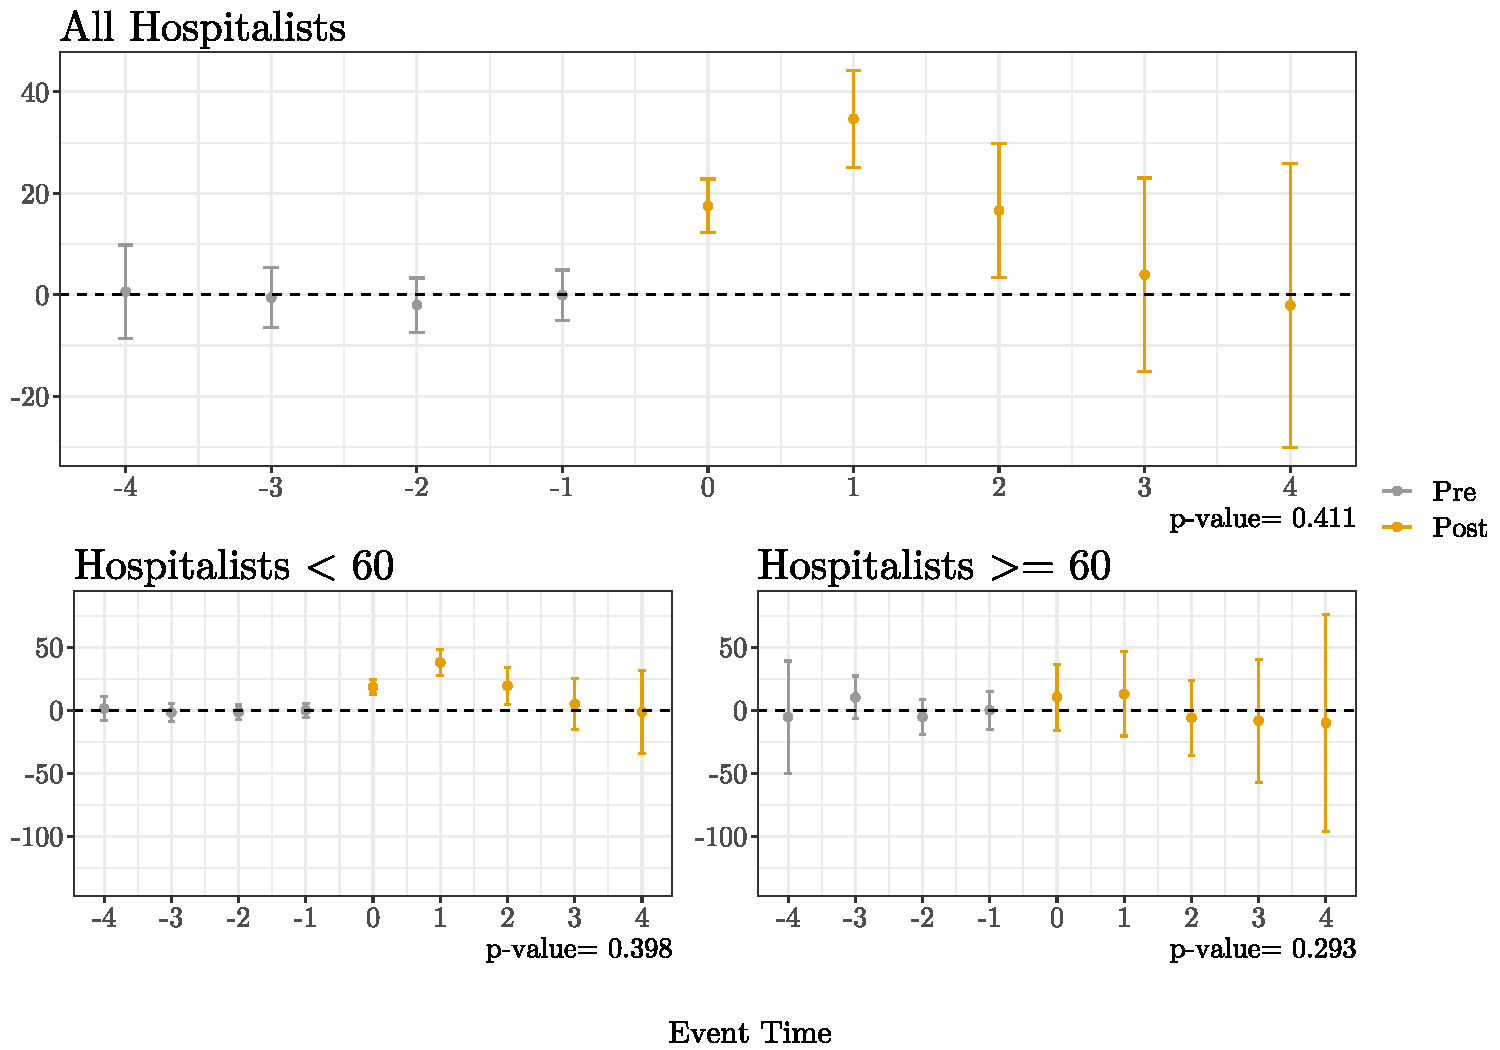
\includegraphics[scale=.6]{Objects/patient_plot.pdf}
    \label{fig:patient}
    \vspace{2mm}
    \caption*{\footnotesize{\textit{Notes:} The top panel shows average group time treatment effects aggregated over groups to an event study plot. The bottom show these results for different subgroups of physicians by age. The p-value listed for each graph corresponds to a Wald test for pre-trends. Confidence intervals shown are simultaneous confidence bands accounting for multiple hypothesis testing. Overall ATT for all, $<$ 60, $>=$ 60 with SE in parentheses: 28 (5.0), 25.6 (5.2), 40.4 (15.0), respectively.}}
\end{figure}

While I am investigating the supply side factors of this outcome, patient count is also driven by demand for health care. A major change in the U.S. health care system, the Affordable Care Act (ACA) was passed in 2010 and took effect in 2014. If my results are driven primarily by the group of hospitals who implemented EHRs in 2014, one might be concerned that the legislation may be driving the increased patient count. The ACA had potentially opposing effects on Medicare patients: they may be crowded out by an increased demand in Medicaid patients, or the small changes to Medicare may have led to an increase in utilization from the Medicare population. A recent study found no negative spillovers to the Medicare population due to the ACA (\cite{carey2020impact}), suggesting that demand change is not driving my results. Additionally, I present average group time treatment effects for each treated group in Figure \ref{fig:patientgroup}. Each group shows the same pattern of an increase in patient count after exposure, suggesting that the groups affected by the ACA are not driving the results. 

\begin{figure}[ht!]
    \centering
    \captionsetup{width=.6\linewidth}
    \caption{Effect of EHR Exposure on Patient Count by Group}
    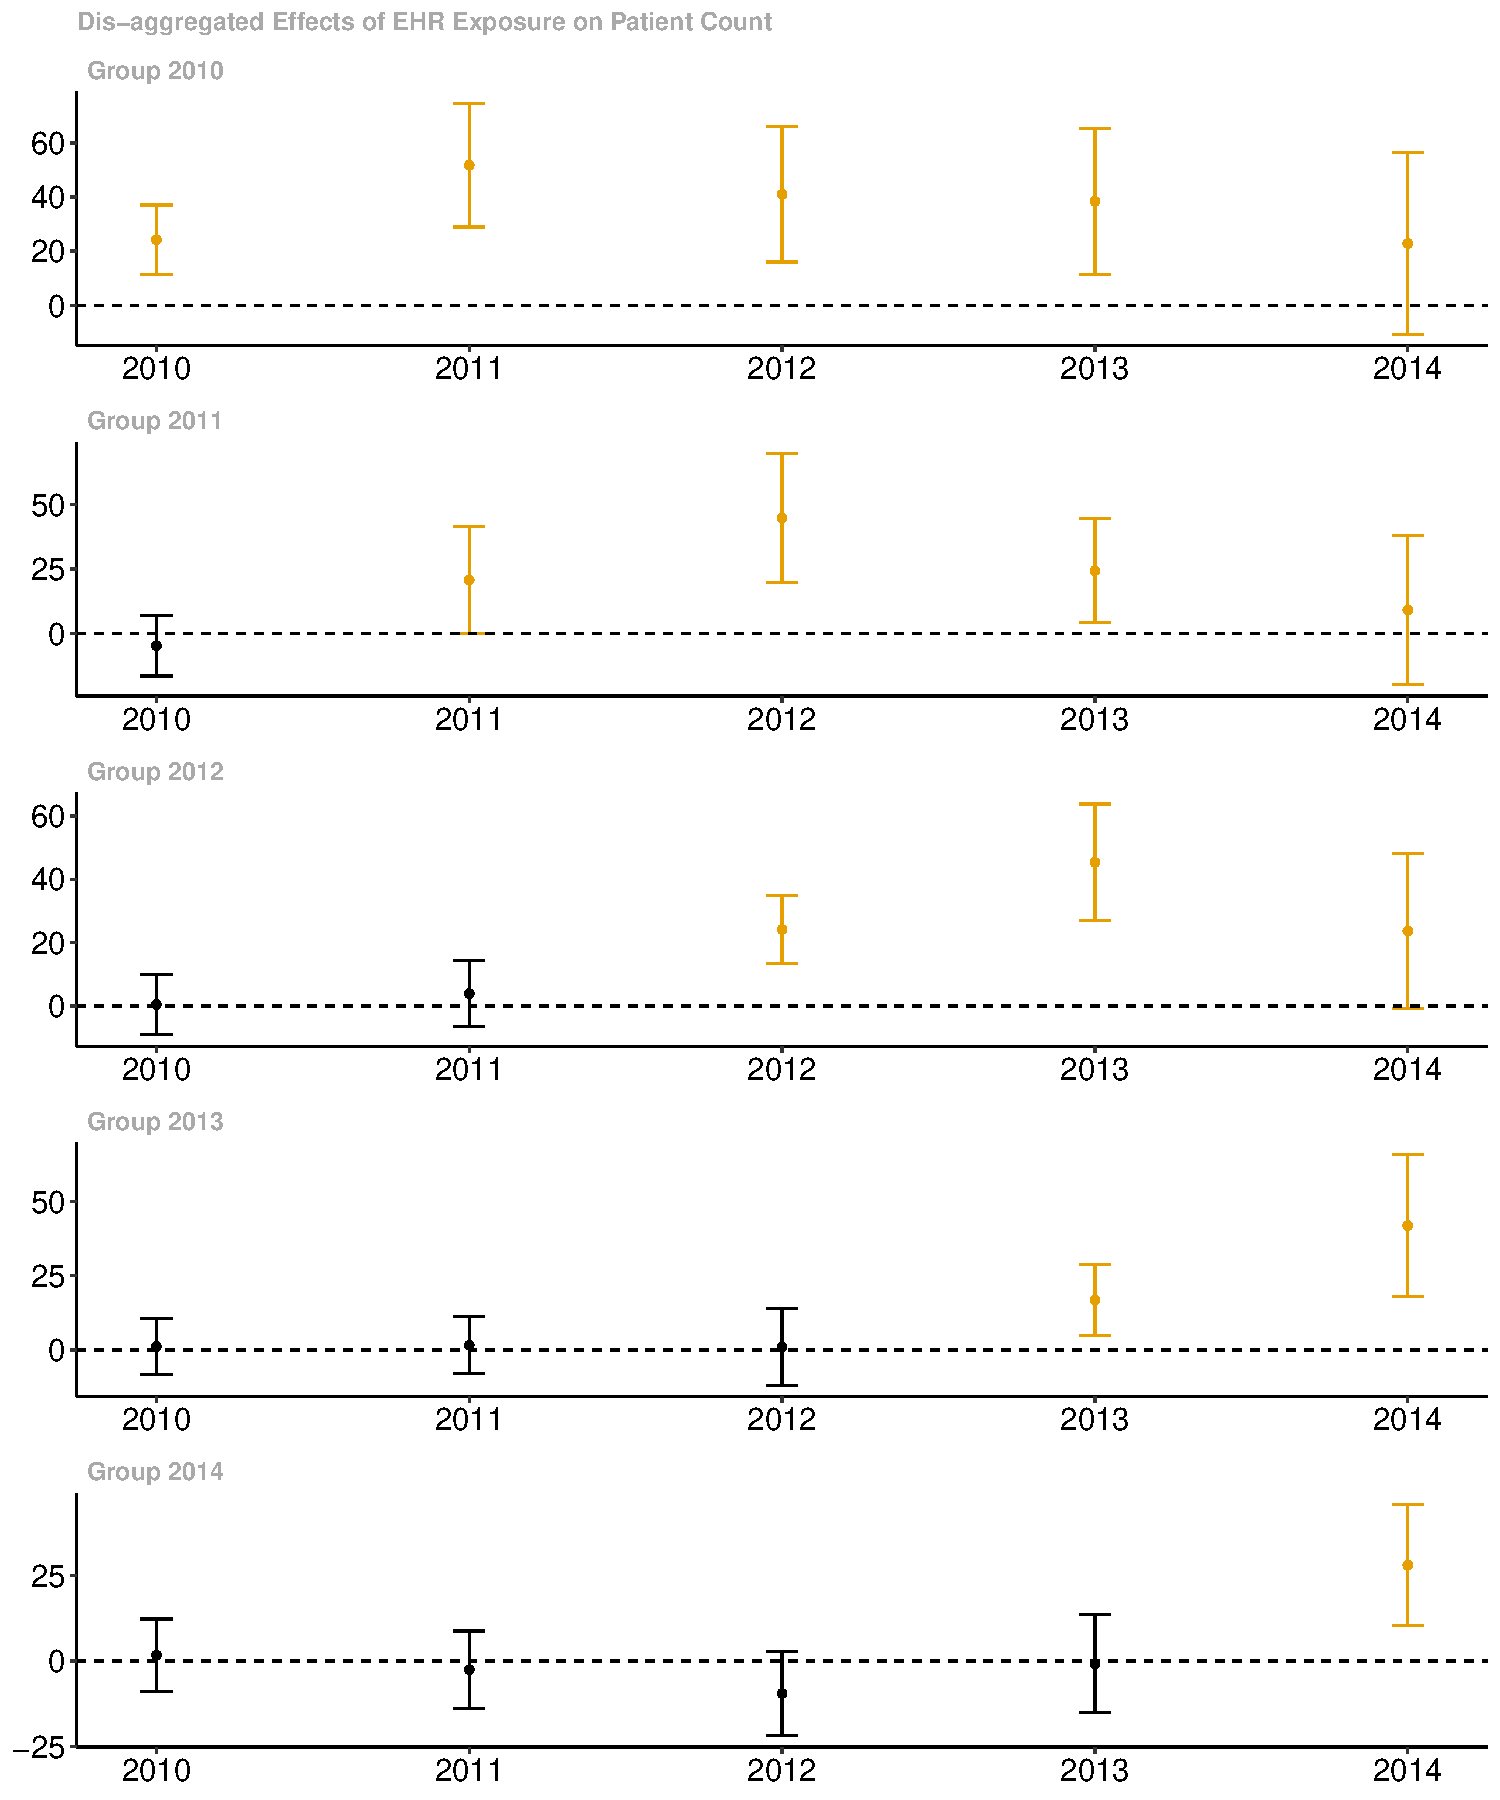
\includegraphics[scale=.47]{Objects/patient_group.pdf}
    \label{fig:patientgroup}
    \vspace{2mm}
    \caption*{\footnotesize{\textit{Notes:} Plot shows average group time treatment effects for each treatment group.}}
\end{figure}

It may be that that EHR exposure affects whether physicians are included in the analysis (since I drop those who retire or move), indicating a nonrandom attrition problem. That is, if productive or tech savvy physicians are the ones who remain in the same hospital after EHR exposure, the estimates are biased.The proportion of those who are not included in this analysis is 18\% in the control group and 36\% in the treated group. To investigate whether my results are robust to this issue, I construct average treatment effect bounds as in  \citeauthor{lee2009training} (\citeyear{lee2009training}). For these bounds to be valid, a monotonicity assumption must hold on selection. That is, treatment can only affect selection in one direction. In my case, that means that EHR exposure increases the likelihood of retiring or moving workplace settings and no physicians remain in the sample under treatment who would have retired or moved in the absence of EHR exposure. Since I find in earlier analyses that physicians are more likely to move and retire due to EHRs, this assumption is reasonable. To compute the bounds, I trim the distribution of patient count in the control group by the difference in attrition rate. Trimming the bottom (top) and taking the differences in expectation between treatment and trimmed control provides a lower (upper) bound. This bounding yields an interval estimate of 54.6 patients to 125.4 patients, compared to the main result of 28 patients. The bound therefore suggests selection of physicians pushes the estimate down.

Similarly, I investigate whether this increase in the number of patients seen is due to the decrease in working physicians. Specifically, a hospital that loses a portion of their physicians, and divides those patients between the remaining physicians. In the long run, the hospital should hire new physicians to replace those that left, but in the short run estimates could be driven by increased workload instead of EHR use. This could explain why there is a much larger increase in the first year after exposure compared to the magnitudes of the estimates as they level out over time. Using the estimates I found in Section \ref{sec:retire}, I calculate the increase in the number of patients that would occur if all patients from retired physicians were divided between remaining physicians. In the year of exposure the entire increase in patient count is due to EHR use since I find no effect on the likelihood of retirement. In the first year after exposure, I estimate the increase in patients due to retiring physicians to be approximately 20 patients, which is less than the observed patient count estimates presented above. However, the second year after exposure is when I observe that largest effect on retirement, and so I do not rule out that the increase in patient count for every year after the first could be caused by the decrease in physicians. 

Finally, I consider whether EHR exposure affects claims filed per patient. On average, physicians file roughly 4 claims per patient. I present estimates in Figure \ref{fig:claim}, which shows that EHRs tend to increase claims filed per patient over time. The magnitude of the effect ranges from .2 to .8, or 5-20\% relative to the mean, indicating that as physicians are exposed to the new software, they bill for more items on average.  I also show heterogeneity of this result by age group, and the bottom panel of Figure \ref{fig:claim} shows that younger physicians are exhibiting more of an increase in claim count than older physicians.

There is no evidence of a pre-trend driving this result, and I also show robustness to violations in parallel trends in Appendix \ref{sec:pretrends}. I also compute \citeauthor{lee2009training} (\citeyear{lee2009training}) bounds for this outcome due to the limited sample. The computed bounds on the average treatment effect are .45 to .6 claims per patient, compared to the overall effect in the main specification of .33. The effect becomes even larger when accounting for a particular type of physician being left in the sample. However, when I analyze this relationship under different data specifications (shown in Appendix \ref{sec:chart}, around half of the estimates are null. Anticipation and limiting sample years cause the effect to disappear or even become negative. Thus, it is not clear whether this positive effect is actually an unintended consequence of EHRs since the effects are not necessarily robust to many specifications. 
      

\begin{figure}[ht]
    \centering
    \captionsetup{width=.85\linewidth}
    \caption{Effect of EHR Exposure on Claims per Patient}
    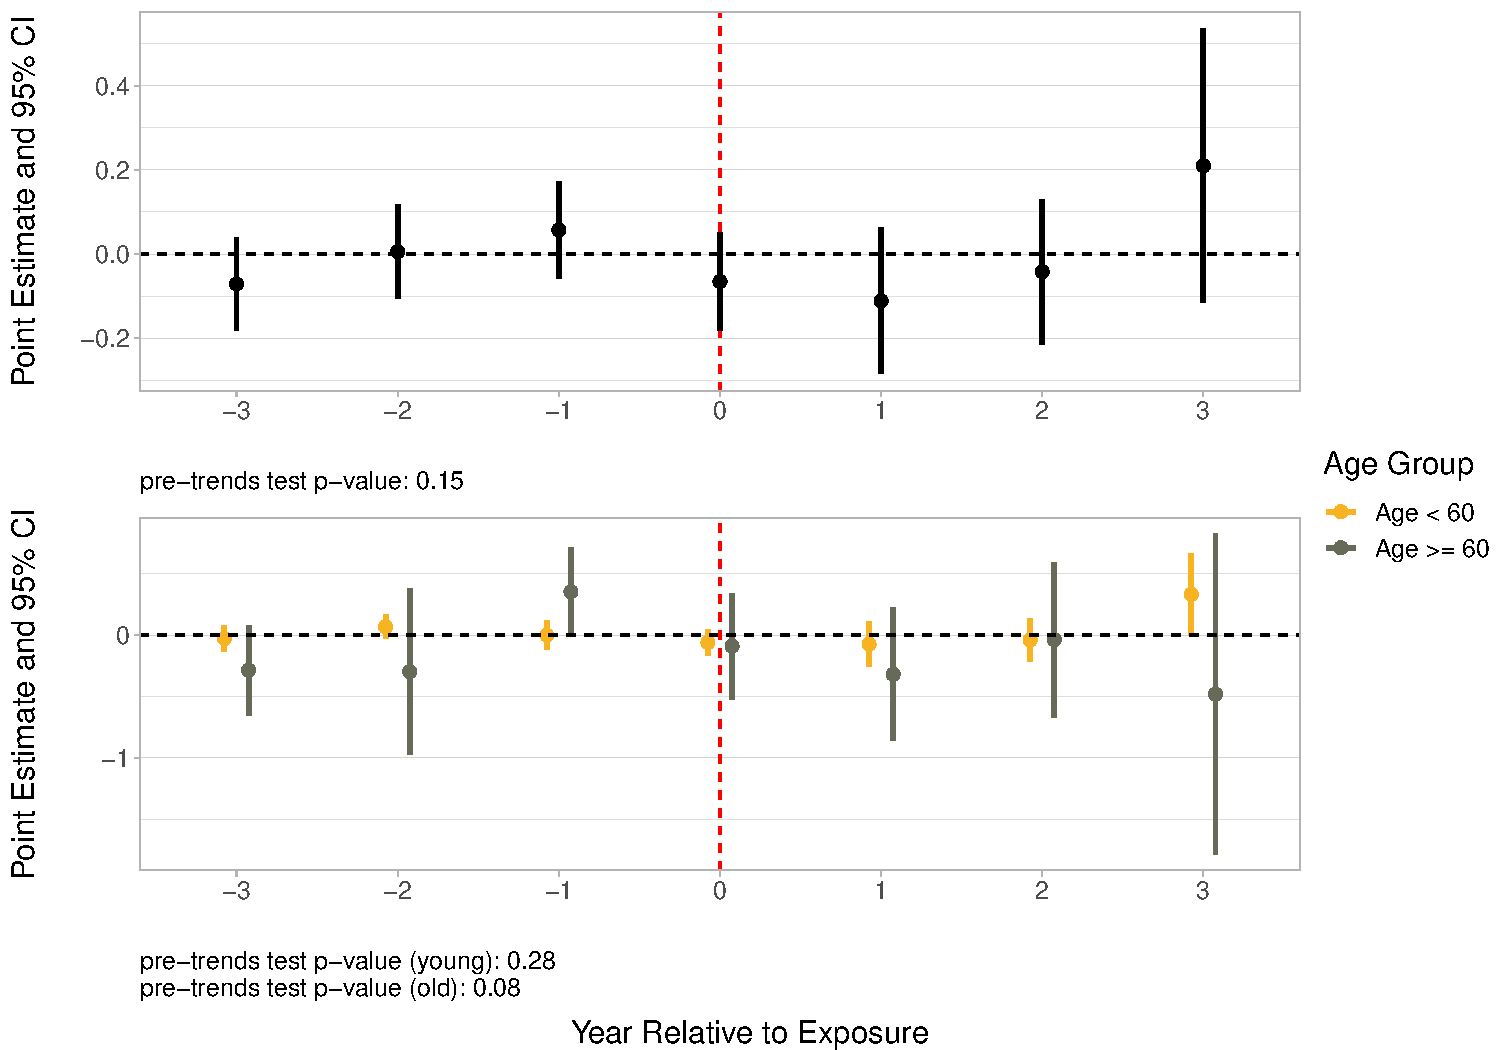
\includegraphics[scale=.6]{Objects/claim_per_patient_plot.pdf}
    \label{fig:claim}
    \vspace{2mm}
    \caption*{\footnotesize{\textit{Notes:} The top panel shows average group time treatment effects aggregated over groups to an event study plot. The bottom show these results for different subgroups of physicians by age. The p-value listed for each graph corresponds to a Wald test for pre-trends. Confidence intervals shown are simultaneous confidence bands accounting for multiple hypothesis testing. Overall ATT for all, $<$ 60, $>=$ 60 with SE in parentheses: .33 (.09), .37 (.08), .05 (.44), respectively.}}
\end{figure}



\section{Physician Influence of EHR Decision in Hospitals}

\subsection{Hiring Data Assistants}\label{sec:dataass}

The effects found in the above analysis may be biased if there is an external event occurring that is correlated with EHR implementation and exposure. The existence or hiring of employees with the purpose of utilizing electronic health records on a physician's behalf is a way for physicians to continue working in a hospital with an EHR but not experience exposure to the technology. Employees of this type are traditionally referred to as scribes, and are assigned a medical tax ID when working in hospitals. They have the following official titles in tax data: Coding Specialist (Hospital Based), Health Information Technologist, and Registered Record Administrator. I refer to any employee in these categories as a data assistant. In this section, I investigate whether data assistants were hired in accordance with EHR implementation and whether the presence of data assistants affects physician response to EHRs. This is particularly relevant for the productivity and efficiency outcomes where I find that EHRs have an effect.  

First, using NPPES data on all NPIs and their tax information, I analyze the existence of data assistants in hospitals. Figure \ref{fig:dataassistant_histogram} presents a frequency plot of the year of activation for every tax code that falls in the categories listed above. The graph is clearly skewed towards later years, where a significant increase in the number of new data assistants occurred in 2014. If hiring data assistants was directly correlated with both EHR implementation and physician frustration, one would expect the increase to occur from 2011-2012, when a majority of physicians first became exposed to EHRs. The results of my main specification are not sensitive to leaving out later years, which is a good indication that the results are not driven by the enumeration of data assistants. 

\begin{figure}[t]
\centering
\captionsetup{width=.5\linewidth}
\caption{Frequency of Data Assistant Enumeration by Year}
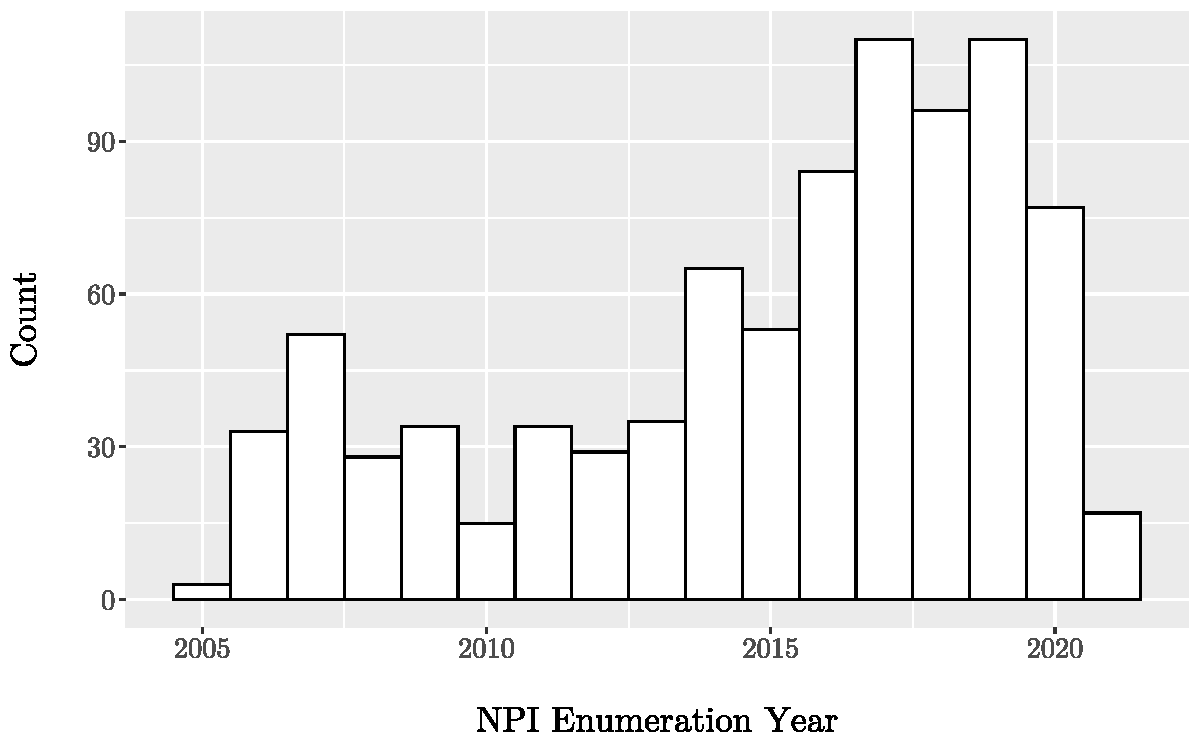
\includegraphics[scale=.5]{Objects/dataassistant_histogram.pdf}
\label{fig:dataassistant_histogram}
\vspace{2mm}
    \caption*{\footnotesize{\textit{Notes:} Histtogram uses NPPES data on the enumeration of certain types of NPIs to estimate the number of new data assistants being hired in each year of my sample.}}
\end{figure}

Further, I investigate the occurrence of physicians and data assistants sharing patients in the CMS Shared Patient data. If data assistants record patient information during appointments, they will be included on the claim to Medicare. I create a list of physician-years for which the hospital has a positive number of shared patients with a data assistant. I merge this to the physician-hospital pairs and create a physician level variable for they are associated with a data assistant. I find that .1\% of physician-year observations are associated with data assistants. This sample of physicians is too small to analyze whether data assistants are more likely with EHR exposure, yielding largely noisy estimates. However, I limit the sample to only physicians not associated with data assistants and find that the magnitude of estimates are similar. Results from specifications where data assistants are excluded are given in Appendix \ref{sec:chart}.

\subsection{Endogeneity of EHR Implementation}\label{sec:endogeneity}

Another way certain physicians may avoid EHR exposure is to exhibit decision making power to either delay or encourage EHR implementation in hospitals. This would make the binary treatment variable endogenous, biasing the results of the main specification, as it includes physicians who are selecting into their own exposure. I address this question by limiting the sample of hospitals, only including those which are considered to have low vertical integration with physicians. That is, physicians are not likely to be in leadership capacities, and thus less likely to be decision makers. I then redefine exposure as when a physician is exposed to an EHR in low integration settings. I present details of how I define integration and results for this specification in Appendix \ref{sec:changes}. In general, group time estimates are similar to those in the main specification, with the exception of the probability of working in an office setting, which may indicate some correlation between EHR adoption in high integration settings and acquisition of physician offices. That mechanism is beyond the scope of this project and left to future research. 


\section{Conclusion}

A technology expected to revolutionize the health care system was the advancement of health information technology in the form of complex electronic health record (EHR) systems. While they have the potential to improve efficiency, cut costs, and improve patient outcomes, these have not come to fruition. While the effect of EHRs on these outcomes has been directly studied, there is a gap in understanding how physicians, the primary user of this technology, responded to their rapid implementation of EHRs. In this study, I analyze the effect of implementing electronic health records on various physician labor market outcomes, since EHRs have been controversial and speculated as a cause of physician burnout. Understanding how physicians respond to this technology is important, as physician labor markets have implications for access to care, quality of care, and costs. 

I utilize data on shared patients between medical entities, hospital EHR use, and physician billing activity to analyze this relationship. Using a difference-in-differences framework, I find that physicians are more likely to leave clinical settings due to EHR exposure, where the magnitude for senior physicians is larger than that for younger physicians. Further, I find evidence that physicians who do not retire change where they work because of EHR exposure, particularly shifting from hospitals towards offices. Finally, physicians who utilize EHRs exhibit an increase in the number of patients seen that cannot fully be explained by redistributing patients or selection of physicians. 

The implications of these results are threefold. First, many physicians left clinical settings in a concentrated number of years due to EHR exposure, potentially worsening patient access to care issues. Second, in a field where younger physicians learn many skills through observing senior physicians, this particular loss of senior physicians may have long term negative effects on patient outcomes, but this is a question left to future research. Third, physicians are exhibiting behavior that suggests they incur switching costs to avoid external burdens. When policymakers consider regulations on physician practice it is important to understand that physicians may take measures to avoid such regulation and incorporate this into the incentives. Finally, these results speak to the ongoing debate of whether EHRs make health care more efficient. My findings suggest that EHRs make physicians more productive through the number of patients they see. However, the limitations of the data prevent a solid understanding of the amount of time spent with patients, so a future research question is whether this increase in productivity is traded off with time spent with patients.  
 




\clearpage

\renewcommand*{\bibfont}{\footnotesize}

\printbibliography

\clearpage


\appendix

\section{Data}\label{app:data}

This section details the process of creating the data set used in the analysis of the main paper. 

\subsection{Physician Specialties by Tax Code}\label{sec:taxcode}

I begin by connecting every National Provider Identifier (NPI)\footnote{Data can be downloaded from \hyperlink{https://download.cms.gov/nppes/NPI/Files.html}{\text{https://download.cms.gov/nppes/NPI-Files.html}}}, an identifier of each medical entity, to a description of their tax code\footnote{Data can be downloaded from \hyperlink{https://nucc.org/index.php/code-sets-mainmenu-41/provider-taxonomy-mainmenu-40/pdf-mainmenu-53}{\text{https://nucc.org/index.php/code-sets-mainmenu-41/provider-taxonomy-mainmenu-40/pdf-mainmenu-53}}}. I then categorize NPIs by key words in their tax code description. Any description containing ``Internal Medicine", ``Hospitalist", ``Family Medicine", or ``General Practice" is classified as a primary care physician (PCP), and any description containing ``hospital" is classified as such. I create two data sets, one containing only PCPs and one containing only hospitals. These data are then used in identifying the relevant NPIs in the CMS Shared Patient Data. 



\subsection{CMS Shared Patient Data}\label{sec:sharedpat}

For years 2009-2015, the CMS collected detailed information on the number of Medicare patients shared between any two NPIs within 30, 90, or 180 day intervals\footnote{Data can be dowloaded from \hyperlink{https://www.nber.org/research/data/physician-shared-patient-patterns-data}{https://www.nber.org/research/data/physician-shared-patient-patterns-data}}. I use data that captures shared patient activity in 30 day intervals. I merge the shared patient data to the filtered tax code data created in Section \ref{sec:taxcode} to identify NPIs who are either PCPs or hospitals. I filter the pairs to include one physician and one hospital; there are 12.6 million of these pairs. Some pairs are duplicates from the hospital being listed first or second in the shared patient data (being listed first means the patient went to NPI 1 first, but my analysis does not depend on the order of care, only the relationship between hospital and physician as a whole). I combine duplicates into one observation, summing the same day count variable. Once duplicates are removed, there are 7.1 million observations. Most of the pairs have very few shared patients, which is not indicative of the physician working inside the hospital. I drop any pairs who do not have at least 30 same-day shared patients per year the pair appears in the data.\footnote{As a sensitivity analysis, I also consider thresholds of 10 and 60. Results are similar and can be found in Figure \ref{sec:chart}.} The final list of pairs consists of 1.3 million observations. 

\subsection{Pair-Level Variables}

I combine the physician-hospital pairs created in Section \ref{sec:sharedpat} with various data sets for hospital or physician level information. First, I merge to CMS Physician Compare\footnote{Data can be downloaded from \hyperlink{https://data.cms.gov/provider-data/dataset/mj5m-pzi6}{https://data.cms.gov/provider-data/dataset/mj5m-pzi6}} for information on each physician's graduation date. This data contains more information on physician quality, but I am limited to time-invariant information since Physician Compare spans 2012-2015 and 2010-2012 is a time of major EHR implementation. I drop any physicians who graduated medical school after 2004, since graduating after that means leaving residency or graduating during the span of my main data, 2009-2017, and potentially exhibiting labor market changes that seem associated with EHRs but are not. 

For hospital level variables, I use an AHA-NPI crosswalk to merge the pairs to the Annual Hospital Administration Survey (AHA Survey) from 2009-2015. From this data I collect information on each hospital's EHR use. There are 4,253 unique AHA hospitals in the shared patient data. I drop any hospitals that aren't in the AHA Survey due to lack of information on EHR use. After limiting the hospitals, there are 780,000 observations of pair-years left. Next, I investigate the hospitals with missing information for EHR use. There are 89 hospitals in the data who never answer the survey question about EHR use; I drop these hospitals. If a hospital does not answer the survey question in one year, but the year before and after have an identical survey answer, I fill in the missing year of information. Then there are 4,253 observations with missing data for the EHR survey question. I make a further limitation to hospitals with at least 10 beds. There are only 58 unique hospitals in the data with less than 10 beds, and these are likely very different from the rest of the sample of hospitals. I sum a physician's same day count over their hospitals in a given year to create a physician level patient count variable. 

Specifically, I use the general survey question about each hospital's EHR use to define my key treatment variable. The survey asks the extent to which the hospital utilizes an EHR and allows for three answers: not at all, partially utilize an EHR, and fully utilize an EHR. I create a binary variable equal to one if the answer is fully utilize, zero otherwise. The data will be aggregated up to the physician level due to physician level outcome variables, so I first transform the pair-level EHR variable into a treatment variable at the physician level. I create a variable capturing the first year that at least one of a physician's connected hospitals uses an EHR. For the endogeneity discussion in Section \ref{sec:endogeneity}, I create a similar variable but only count a physician as exposed if a hospital categorized as "low-integration" adopts an EHR. The level of vertical integration between hospital and physician is defined as in \citeauthor{dynan1998assessing} (\citeyear{dynan1998assessing}) using the organization type of the hospital. Hospitals classified as IPA or PHO are low-integration, and any other type is high integration. Finally, the last variable I create before aggregating to the physician level is an indicator for whether the physician works with the same set of hospitals through the entire sample. I create this variable by comparing a physician's number of hospitals in each year to the maximum number of hospitals they ever work with. If there is any year in which the a physician's number of hospitals is less than the maximum number of hospitals they ever work with, the indicator for never having a new NPI is set to 0. I use this variable to limit the sample in Section \ref{sec:patientcount}. 

Finally, I aggregate to the physician level by only keeping variables that do not vary by hospital. The variables in the physician level data are year, physician NPI, graduation year, years of experience, number of hospitals, minimum year exposed to EHR, minimum year exposed to EHR in low integration hospital, number of systems, and never works with a new NPI. I complete this data to include years 2016 and 2017, but leave time varying variables missing for those years. Thus, this is a balanced panel of physicians. I save this data to be merged with physician labor market activity in Section \ref{sec:appmdppas}.

\subsection{Physician Labor Market Activity}\label{sec:appmdppas}

Using physician NPI, I merge the physician treatment data to Medicare Data on Provider Practice and Specialty (MD-PPAS)\footnote{Information on data located at \hyperlink{https://resdac.org/cms-data/files/md-ppas}{https://resdac.org/cms-data/files/md-ppas}}, which spans 2009-2017. This data contains variables on physician specialty, Medicare claim counts in various zip codes, unique number of patients seen, fraction of patients seen in specific settings, patient demographics, and physician date of birth. Once the data is merged, I make a further limitation to drop any physicians with less than 70\% of their total patients in a hospital setting.\footnote{I consider different thresholds as a sensitivity analysis. The results are similar, and can be found in Section \ref{sec:chart}} This limitation is to continue ensuring that I am focusing on physicians working in hospitals who will be subject to their EHR use. With this limitation, there are approximately 214,000 observations left in the data. 

Next, I create the dependent variables used in the analysis. The first outcome is whether a physician chooses to retire or not. First, I sum a physicians claim counts across zip codes into one variable for total claim count in a given year. Then, I create a variable that sums up a physicians claims in all future years. In 2009, this variable sums up all claims from 2010-2017, and so on. Then I create a variable for the first year that a physician has a future claim count of zero. However, this counts retirement one year too early. For example, if a physician has no claims from 2014 to 2017, the minimum year variable is set to 2013, but the first year of retirement is 2014. Thus, I add one year to the minimum year variable. I then define the outcome variable, retire, as one if a physician ever retires and the year is equal to the first year of retirement. I also create a physician level variable for whether they ever retire for sample limitations in analyzing other outcomes. 

The next outcome variables consider level of labor market activity in office settings. The first decision to make is how to handle years where a physician has missing data for claims. A year of missing data can mean the physician had no claims that year, or the observation was removed due to insufficient claims (less than 11). A conservative assumption is to assume a year of missing data means zero claims, thus, I set all missing claim counts to zero. The data already contains a variable for the fraction of patients seen in an office setting, which is used in the analysis, but I further create an indicator variable for whether the physician sees any positive amount of patients in an office setting. Finally, the variables for unique patient count and claim count are already defined. I simply divide the number of claims by the number of patients to get the claims per patient variable used in the analysis. This is the final data used in the paper, with approximately 215,000 observations. 



\section{Sensitivity Analysis}

\subsection{Analyzing Pre-Trends Assumptions}\label{sec:pretrends}

Work by \citeauthor{rambachan2019honest} (\citeyear{rambachan2019honest}) reveals the need to carefully assess the parallel trends assumptions commonly used in difference in difference designs. In my main specification I assume that, conditional on covariates, average outcomes for those treated in group $g$ would have followed a parallel trend as those in groups treated in later periods. I assess this assumption by testing whether the coefficients showing the effect of EHR exposure on an outcome prior to actual treatment are jointly zero. All main specification graphs show p-values from this test. In most analyses, I fail to reject the null that there does not exist a pre-trend. Yet, in some cases, I reject this null. This section utilizes the tools established by \citeauthor{rambachan2019honest} (\citeyear{rambachan2019honest}) to demonstrate robustness of the results found in the main specification, and to investigate whether an effect exists in the cases where a pre-trend may be driving results. 

\subsubsection{Retirement} 

First, I consider the estimated effect of EHR exposure on retirement. While visually there does not appear to be a strong pre-trend, for the full sample of physicians and physicians $< 60$, the p-value indicates a pre-trend may exist. I present a plot of robust confidence intervals under various possible assumptions of parallel trends violations for one year after exposure in Figure \ref{fig:pre_retire}. The original confidence interval is shown in yellow, and in gray are confidence intervals robust to varying functions of parallel trend violations. As I allow for different assumptions on parallel trends, the confidence intervals become larger and contain zero. Under linearity of pre-trend, the confidence interval contains zero but is more similar to the effect found in the main result. This is true for both event time 1 and event time 2. 

\begin{figure}[ht]
    \centering
    \captionsetup{width=.5\linewidth}
    \caption{Retire Pretrends Plot}
    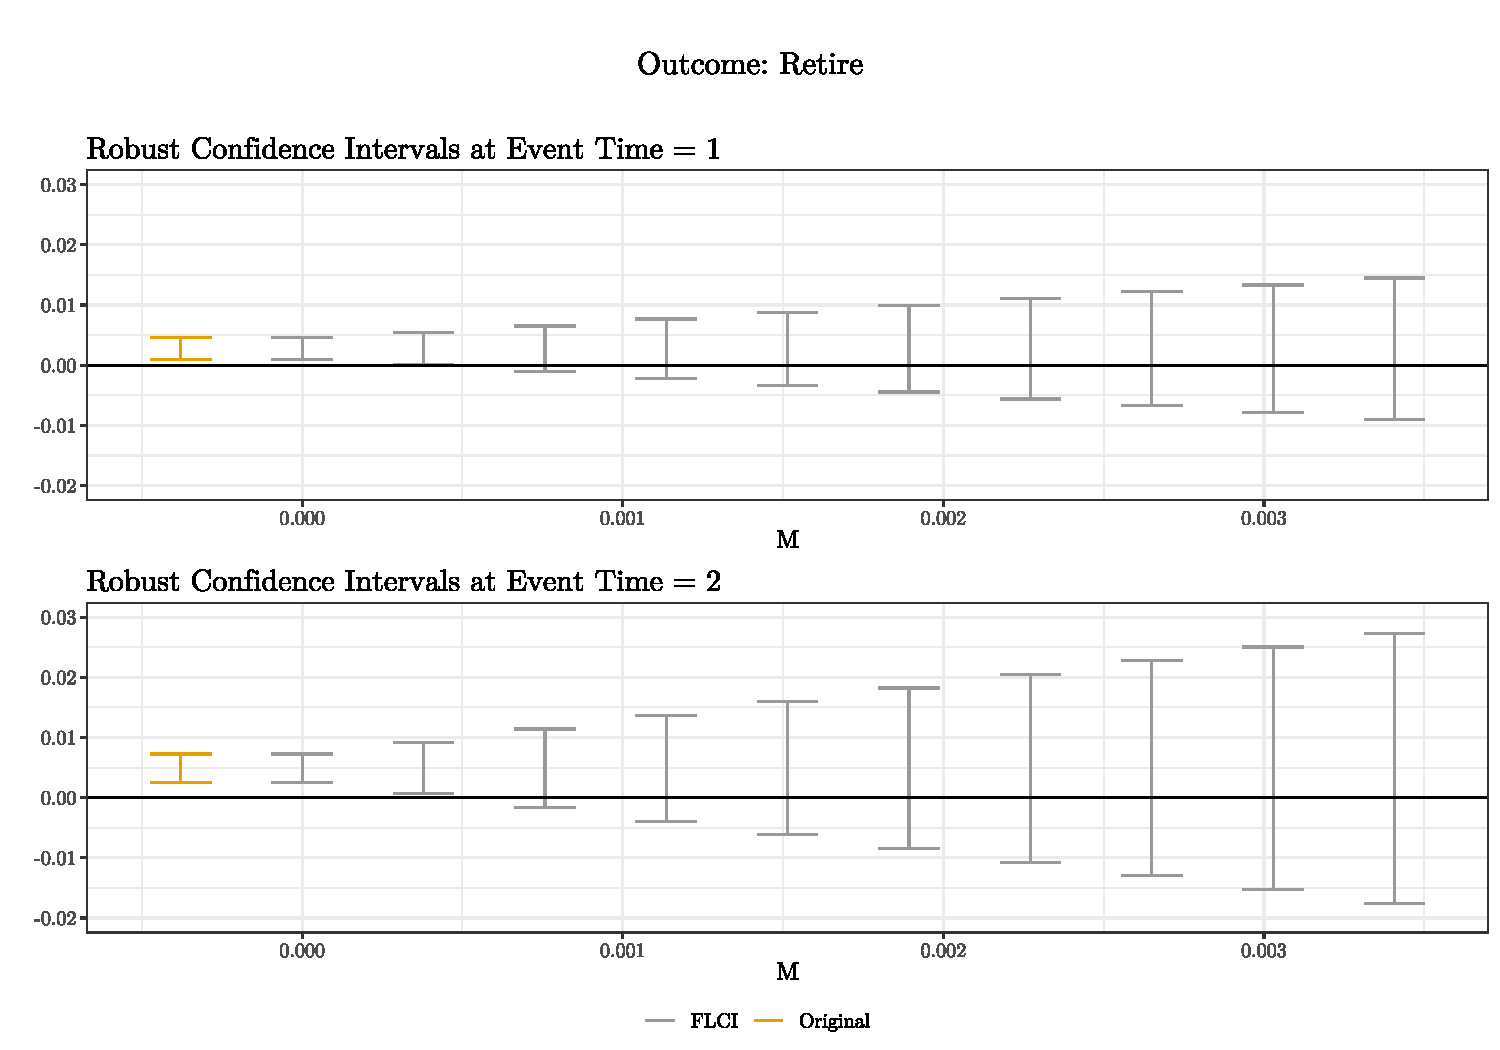
\includegraphics[scale=.5]{Objects/retire_pretrends_plot.pdf}
    \label{fig:pre_retire}
    \vspace{2mm}
    \caption*{\footnotesize{\textit{Notes: This plot shows average treatment effects one year after EHR exposure under different trend assumptions. M=0 indicates a linear pre-trend.}}}
\end{figure}

\subsubsection{Work in Office Likelihood}

Next, I examine pre-trends for the outcome variable indicating whether the physician does any work in an office. The p-values do not indicate pre-trends for the full sample or for physicians $< 60$, but I reject no pre-trends for physicians of retirement age. I show robust confidence intervals for the average treatment effect in the first year after exposure in Figure \ref{fig:pre_work}. For various assumptions on the form of pre-trends, the positive effect holds.

\begin{figure}[ht]
    \centering
    \captionsetup{width=.5\linewidth}
    \caption{Work in Office Indicator}
    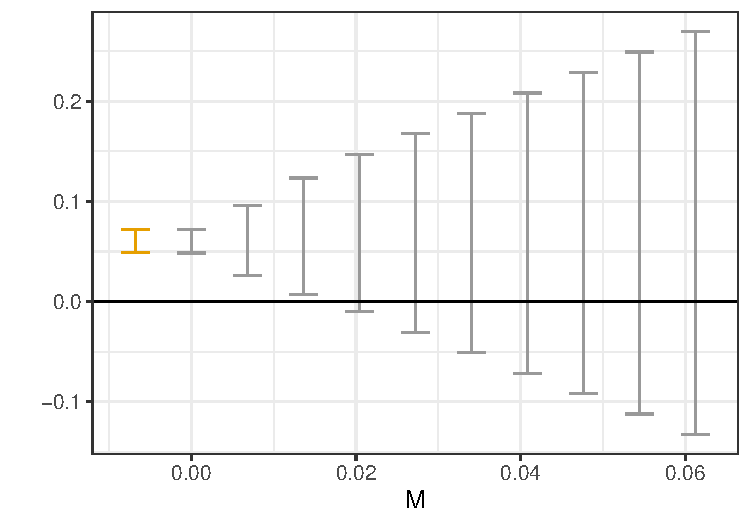
\includegraphics[scale=.5]{Objects/office_ind_pretrends_plot.pdf}
    \label{fig:pre_work}
    \vspace{2mm}
    \caption*{\footnotesize{\textit{Notes: Notes: This plot shows average treatment effects one year after EHR exposure under different trend assumptions. M=0 indicates a linear pre-trend.}}}
\end{figure}

\subsubsection{Fraction of Patients in Office}

The next outcome considered is the fraction of patients seen in an office setting. All p-values suggest there are no pre-trends. I show robust confidence intervals for the average treatment effect in the first year after exposure in Figure \ref{fig:pre_frac}. For various assumptions on the form of pre-trends, the positive effect holds.

\begin{figure}[ht]
    \centering
    \captionsetup{width=.5\linewidth}
    \caption{Fraction of Patients Seen in Office}
    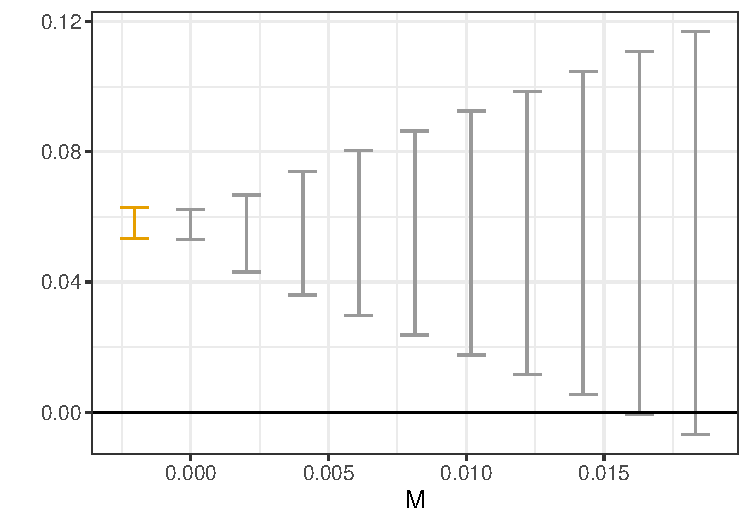
\includegraphics[scale=.5]{Objects/office_frac_pretrends_plot.pdf}
    \label{fig:pre_frac}
    \vspace{2mm}
    \caption*{\footnotesize{\textit{Notes: This plot shows average treatment effects one year after EHR exposure under different trend assumptions. M=0 indicates a linear pre-trend.}}}
\end{figure}

\subsubsection{Patient Count}

Now I examine the sensitivity of the main specification results where the outcome considered is the number of patients seen. None of the p-values indicate a violation of parallel trends, but I present a plot of confidence intervals robust to specified variations in parallel trends as a robustness check in Figure \ref{fig:pre_patient}. This plots indicate that, even under nonlinear deviations in parallel trends, there is a positive effect of EHR exposure on patient count with similar magnitude to that of the main specification.  

\begin{figure}[ht]
    \centering
    \captionsetup{width=.5\linewidth}
    \caption{Patient Count}
    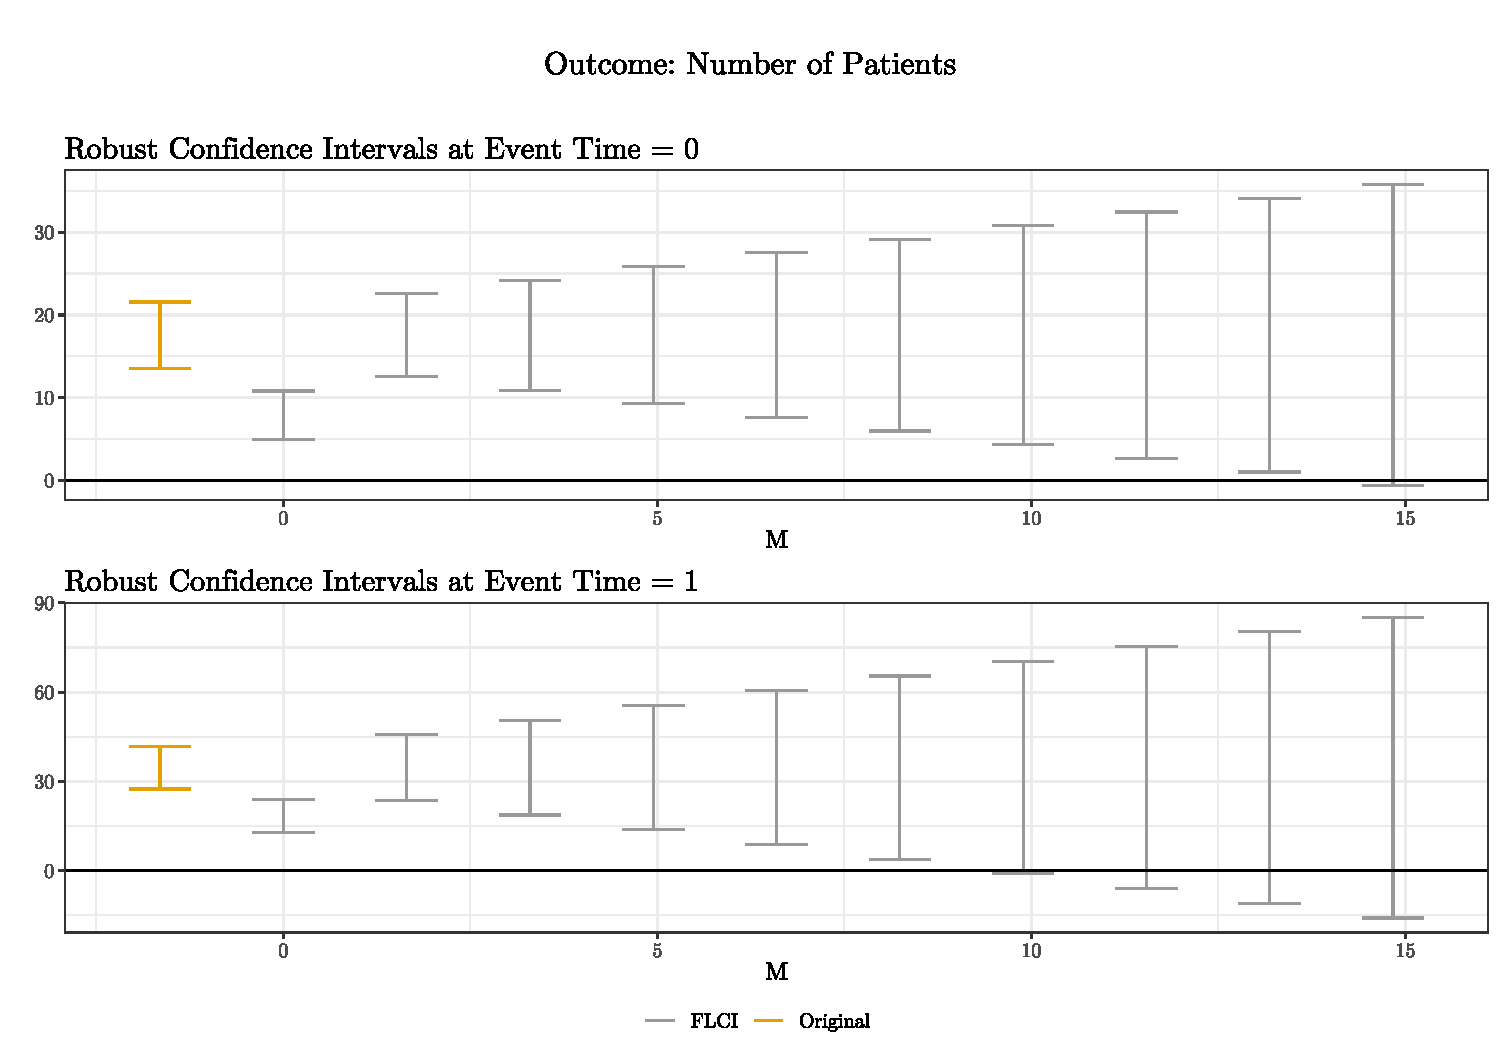
\includegraphics[scale=.5]{Objects/patient_pretrends_plot.pdf}
    \label{fig:pre_patient}
    \vspace{2mm}
    \caption*{\footnotesize{\textit{Notes: This plot shows average treatment effects one year after EHR exposure under different trend assumptions. M=0 indicates a linear pre-trend.}}}
\end{figure}

\subsubsection{Claim Count}

Finally, I assess the results found in the main specification for the outcome variable claim count. The main specification indicates an increase in claims per patient after EHR exposure, but under various specification changes this effect becomes null. Under linear assumptions of a pre-trend form, the effect is similar to that of the main specification. Once more non-linearity is allowed, the effect becomes null. 

\begin{figure}[ht]
    \centering
    \captionsetup{width=.5\linewidth}
    \caption{Claims per Patient}
    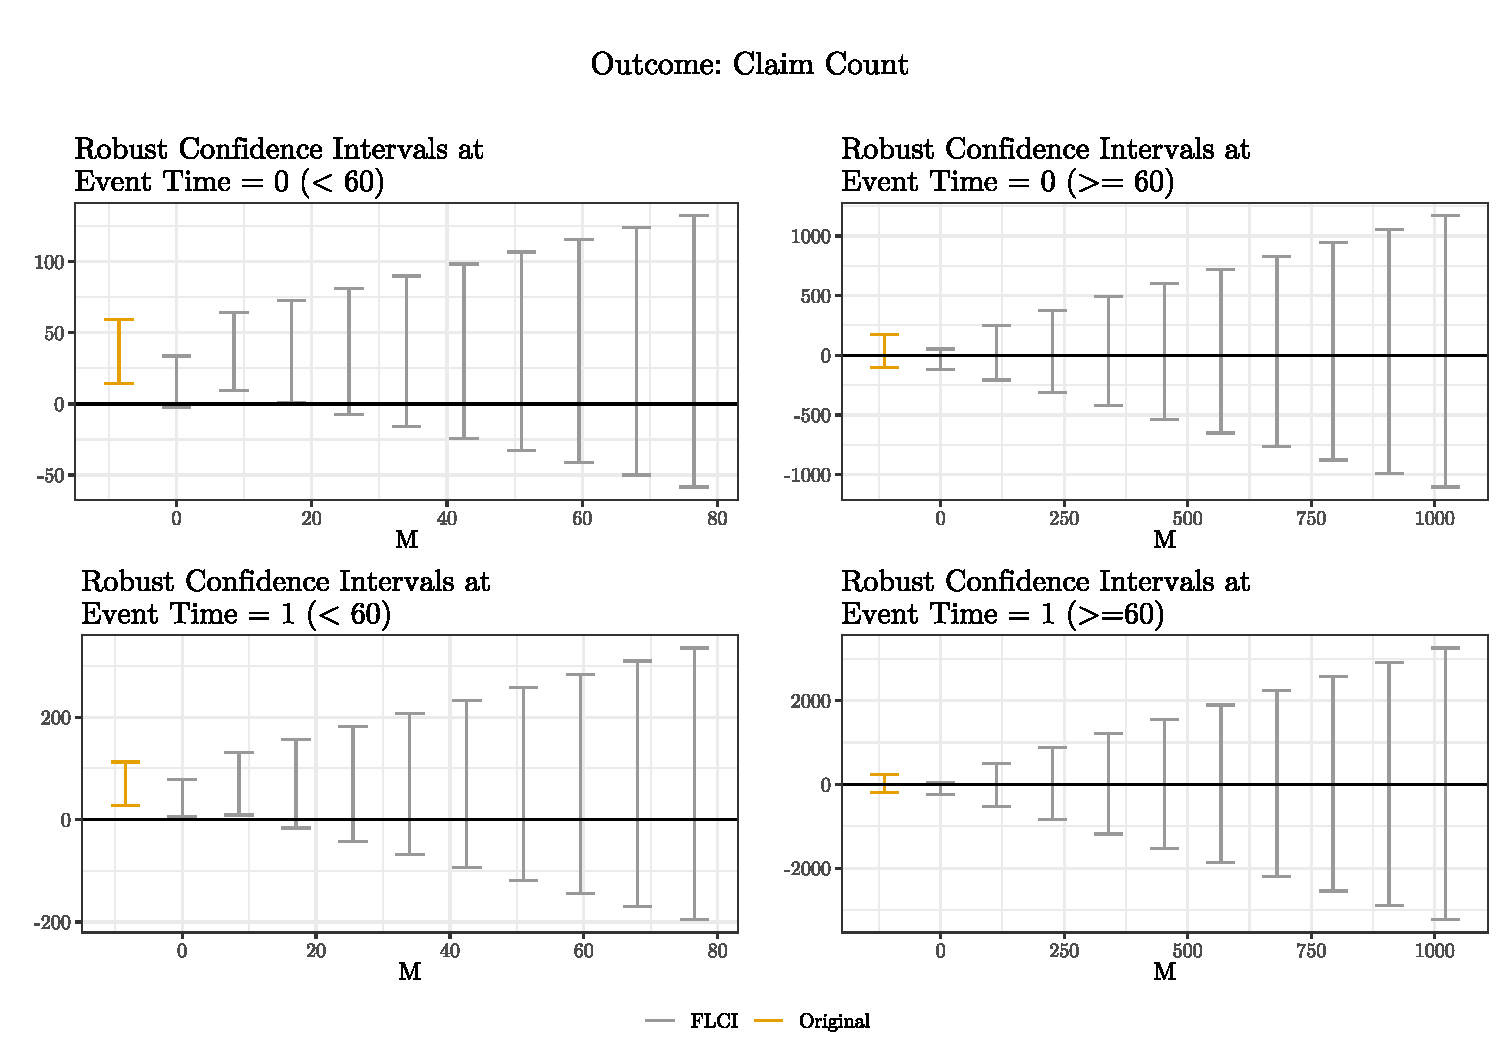
\includegraphics[scale=.5]{Objects/claim_pretrends_plot.pdf}
    \label{fig:pre_claim}
    \vspace{2mm}
    \caption*{\footnotesize{\textit{Notes: This plot shows average treatment effects one year after EHR exposure under different trend assumptions. M=0 indicates a linear pre-trend.}}}
\end{figure}

\subsection{Various Changes to Specification}\label{sec:changes}

For each outcome, there are various adjustments I make to the main specification in order to show robustness. Some of these changes address potential endogeneity concerns, while some provide evidence that the results do not depend on thresholds which may be arbitrary. I will outline each of these adjustments and then present specification charts which account for different combinations of these changes. 


First, I assess the assumption that exposure to an EHR is exogenous to the physician. The main specification of the paper defines a binary treatment variable for whether a physician is exposed to an EHR in any hospital they work in. These results are biased if physicians endogenously select whether they are exposed to EHRs, particularly by participating in the hospital's decision to implement. The results do not indicate that this is a huge issue on average, since we would expect physicians not to respond on the margin of retirement or switching work setting if they are choosing to be exposed to EHRs. Especially in larger hospitals, this is unlikely to occur as an individual physician will not have much input to high level decisions. However, as an attempt to provide more evidence of labor market changes as a result of EHR exposure, I provide results for specifications with an alternate binary treatment variable: whether a physician has been exposed to an EHR in a hospital considered to have low vertical integration with physicians. 

I define a hospital's level of integration based on organizational structure, where independent practice associations (IPAs) and physician-hospital organizations (PHOs) are classified as low vertical integration and other organization types are classified as high vertical integration (\cite{dynan1998assessing}). 



While there is evidence to suggest the time it takes to implement an EHR does not exceed one year, there still may be some anticipation if physicians are expecting implementation in the hospitals they work in. Thus, the specification charts that I present in Section \ref{sec:chart} include specifications where one year of anticipation occurs. 


In the main sample, I define dependent variables using years 2009 to 2017 and drop any physicians who were not exposed to an EHR by 2015 due to data constraints. This leads to estimation based on not yet treated units, because all never treated units are dropped. As a robustness check, I limit sample years to 2009-2015 and use never treated units as the control group. 

As discussed in the body of the paper, I address potential concerns that the hiring of new employees may be driving the results for productivity and efficiency. Thus, as another specification, I restrict the data to only include physicians who have no record of working with data assistants as described in Section \ref{sec:dataass}. 

There are two main thresholds I define in the data process that were arbitrarily chosen. Thus, I present alternate specifications that adjust these thresholds. First, when deciding which hospitals a physician is working closely with, I drop any pairs that fall below 30 shared patients per year. The goal of this threshold is to eliminate pairs for which the physician does not have close ties to the hospital. In alternate specifications, I lower the threshold to 10 patients per year and raise the threshold to 60 patients per year. Second, I only want to include hospitalists in the analysis, and thus drop any physicians that fall below 70\% of patients in an inpatient setting. In alternate specifications, I change this threshold to 50\% and 90\%. While these are still arbitrary, they provide some evidence that changing the threshold does not dramatically change the results. 


\subsection{Specification Charts}\label{sec:chart}

I present overall average treatment effects for each outcome variable under different combinations of the specification adjustments discussed in Section \ref{sec:changes}. On each chart, the main specification is labeled in green and the average confidence bands across all combinations is shown as an orange band. 

\subsubsection{Retirement}

The specification chart for the retirement outcome is presented in Figure \ref{fig:retire_chart}. The main specification yields an average treatment effect of .0025 (significant at all levels). This coefficient is on the higher end of coefficients from all combinations of specifications. However, almost all of the coefficients are positive. Some noisy estimates are to be expected when there are multiple limitations placed on the data. The average confidence interval for all combinations is (.001,.003), so the main specification lies in this interval. These results support my main finding that EHR exposure positively affects the likelihood of retirement among physicians. 

\begin{figure}[ht]
    \centering
    \caption{Outcome: Retire}
    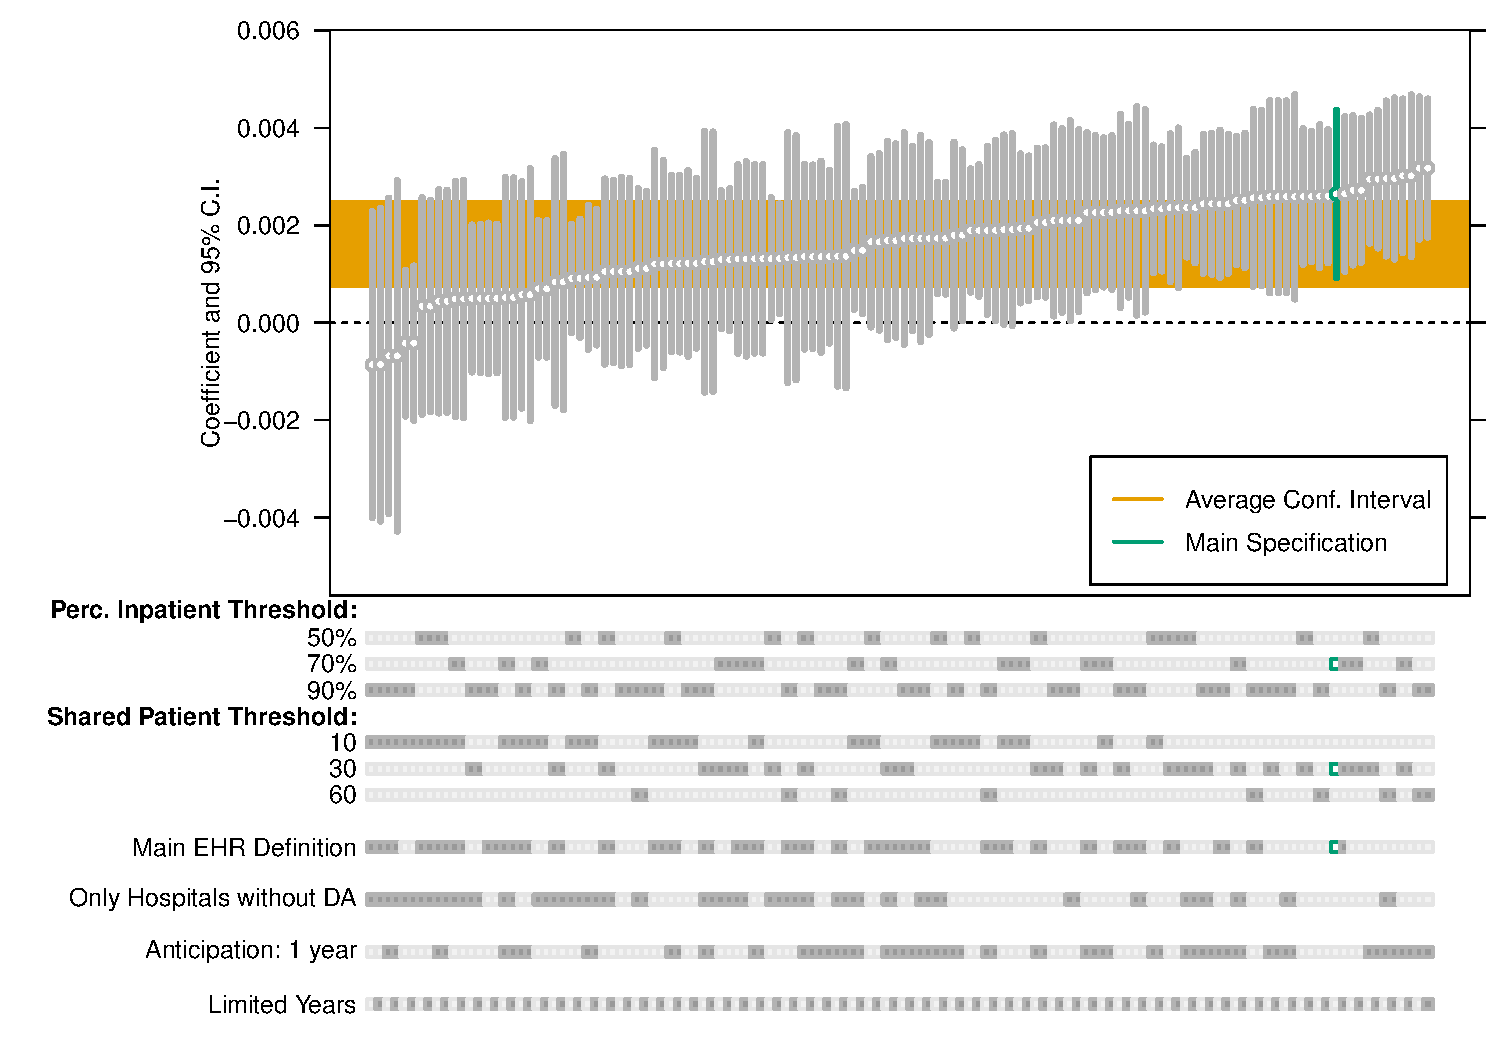
\includegraphics[scale=.7]{Objects/retire_chart.pdf}
    \label{fig:retire_chart}
\end{figure}

\subsubsection{Change Work Setting}

The specification charts for outcomes work in office and fraction of patients seen in office are presented in Figures \ref{fig:work_chart} and \ref{fig:fracoffice_chart}, respectively. First, I discuss the overall average treatment effect of EHR exposure on the likelihood of working in an office. The main specification yields finding that EHR exposure leads to a .07 ppt increase in the likelihood of working in an office. This is on the high end of all combinations of changes to specification, but all reveal a positive effect. On average, the confidence interval falls between .035 and .06. This supports the finding that EHR exposure positively affects the likelihood of working in an office.  

Specification changes that seem to affect the magnitude of the estimate are whether I limit the sample years and which EHR definition is used as the treatment variable. Neither of these change the sign of the estimate, but both limiting sample years and using the low-integration definition of EHR exposure push the magnitude slightly down.  

\begin{figure}[ht]
    \centering
    \caption{Outcome: Work in Office}
    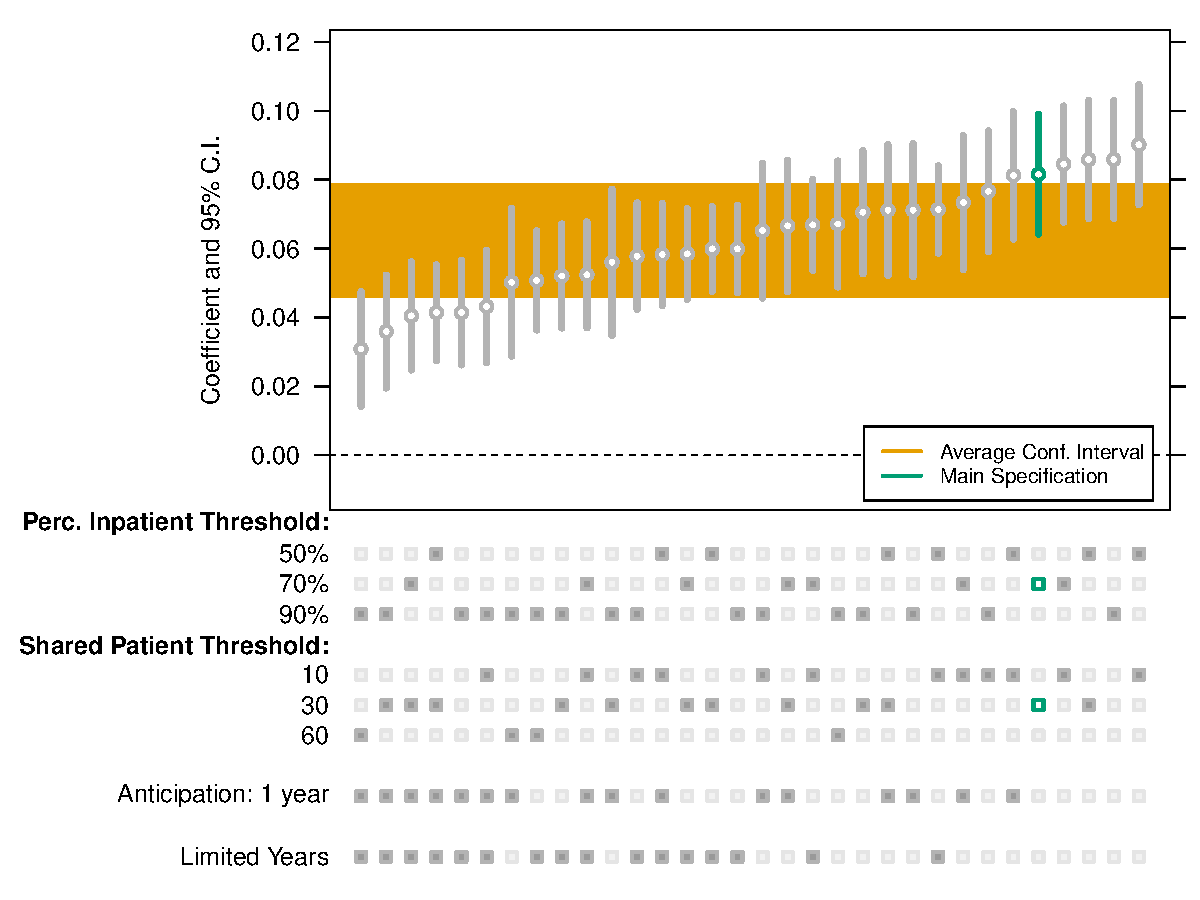
\includegraphics[scale=.7]{Objects/office_ind_chart.pdf}
    \label{fig:work_chart}
\end{figure}

Now I discuss the results for whether physicians change the fraction of patients seen in an office setting due to EHR exposure. Similarly, the ATT from the main specification is on the high end of other ATTs found, but all estimates suggest a positive effect. The average of all the confidence intervals found is (.02, .06), suggesting a positive effect on fraction of patients seen in an office. Changes that affect the magnitude of the estimate (but not the sign) are limiting sample years and anticipation. Limiting the years in the sample and allowing for one year of anticipation both push the magnitude of the estimate down. 

\begin{figure}[ht]
    \centering
    \caption{Outcome: Fraction of Patients in Office}
    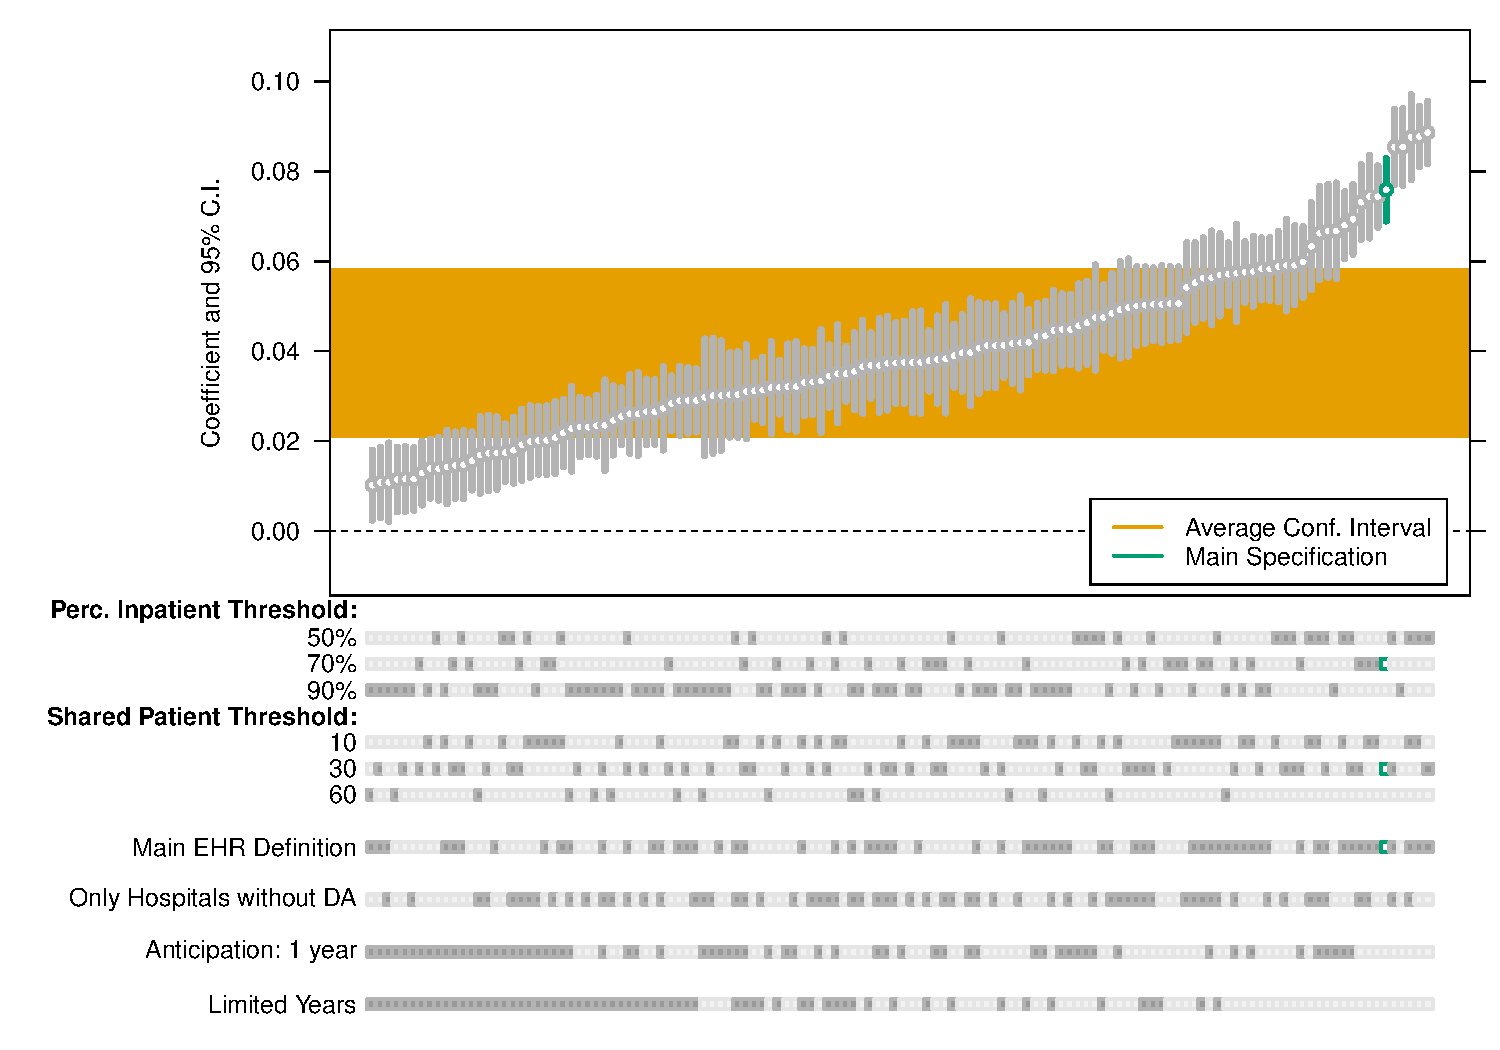
\includegraphics[scale=.7]{Objects/office_frac_chart.pdf}
    \label{fig:fracoffice_chart}
\end{figure}


\subsubsection{Patient Count and Claims per Patient}

In Figure \ref{fig:pat_chart}, I present estimates and confidence intervals for different combinations of specification changes. The results from the main specification is that EHR exposure increases patient count by 28. While most specifications yield positive estimates, about a third of the specifications have a confidence interval that includes zero. It doesn't seem as though any specific change is driving the null result, so I hypothesize that it is due to the reduction in observations due to data limiting. The average of all of the confidence intervals is 7 to 23, indicating that a positive effect on patient count is reasonable. 

\begin{figure}[ht]
    \centering
    \caption{Outcome: Patient Count}
    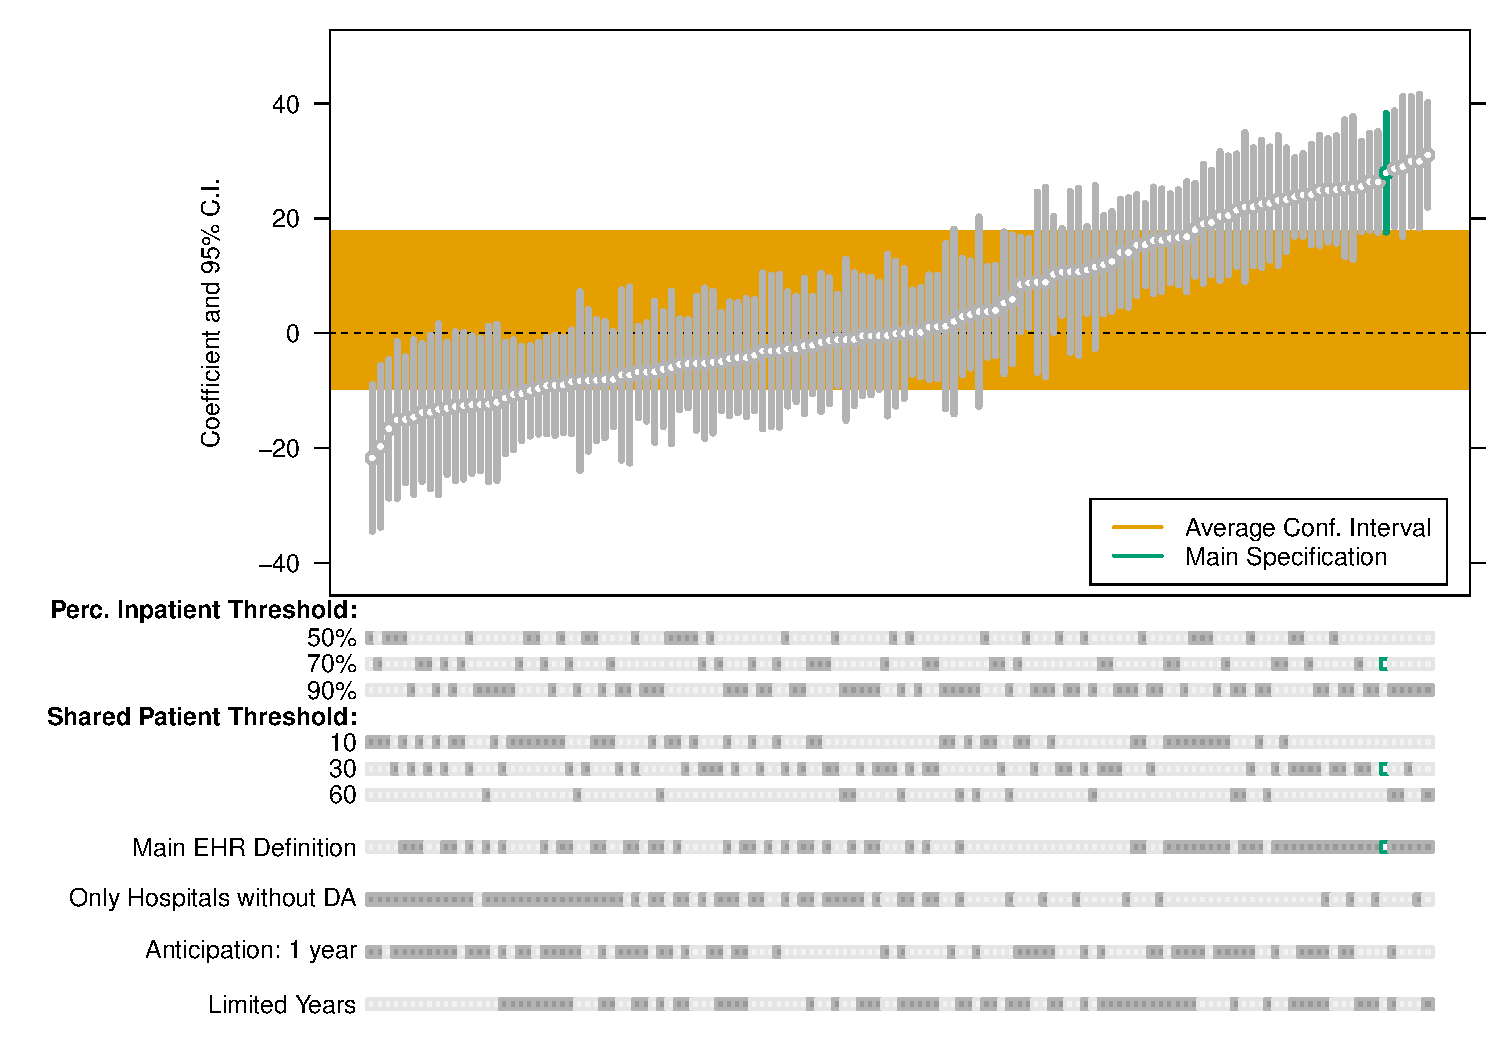
\includegraphics[scale=.7]{Objects/patient_chart.pdf}
    \label{fig:pat_chart}
\end{figure}

Lastly, I examine a chart of estimates for different specifications attempting to capture the effect of EHR exposure on claims per patient. My main finding is that EHR exposure increases claims per patient by around .3. However, various robustness checks reveal that this is overestimated. That is supported in this specification chart as well, where around half of the estimated confidence intervals include zero. Thus, I make no conclusion that EHR exposure increases claims per patient. 

\begin{figure}[ht]
    \centering
    \caption{Outcome: Claims per Patient}
    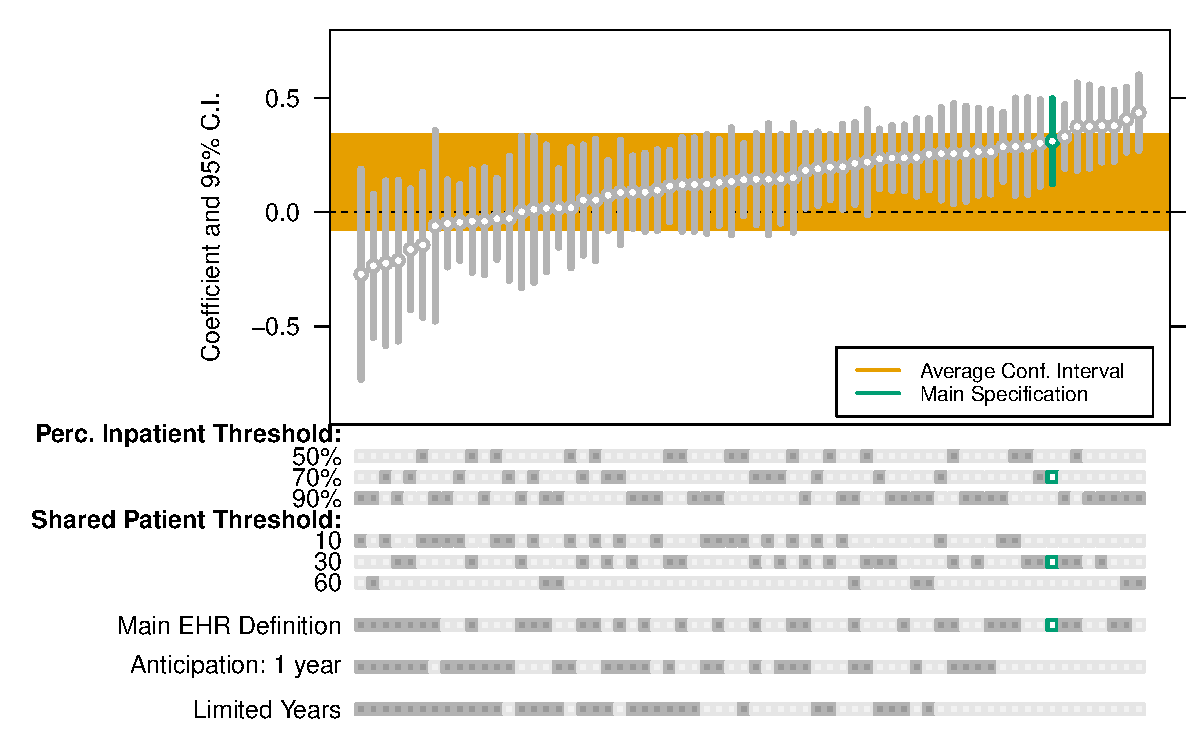
\includegraphics[scale=.7]{Objects/claim_chart.pdf}
    \label{fig:cpp_chart}
\end{figure}



\subsection{Alternative Estimators}\label{app:estimators}

There is a robust recent literature considering the issues with estimating heterogeneous treatment effects with a two way fixed effects specification, the classic approach in staggered treatment setups. To avoid these problems, in my main specification I use the average group time effect estimator established in \citeauthor{callaway2021difference} (\citeyear{callaway2021difference}). In this section, I discuss other potential estimators and why I ultimately included average group time treatment effects as the main specification. 

Before I present these estimators, I present results from a two way fixed effects setup that may suffer bias from negative weighting. Specifically, I estimate the following equation:
$$\text{outcome}_{i,t}=\sum_{j=-4}^{-2} \text{rel\_year}_{j} + \sum_{j=0}^{4} \text{rel\_year}_{j} + \delta_i + \gamma_t,$$
where outcome$_{i,t}$ is one of the five outcomes discussed previously, rel\_year$_j$ is an indicator equal to 1 if year $t$ is $j$ years relative to expansion, $\delta_i$ are physician fixed effects, and $\gamma_t$ are year fixed effects.
These results from each outcome are presented in Figure \ref{fig:twfe}. These results show similar patterns to the main specification, with slight variations in magnitude. 

\begin{figure}
    \centering
    \captionsetup{width=.8\linewidth}
    \caption{Results: Two Way Fixed Effects}
    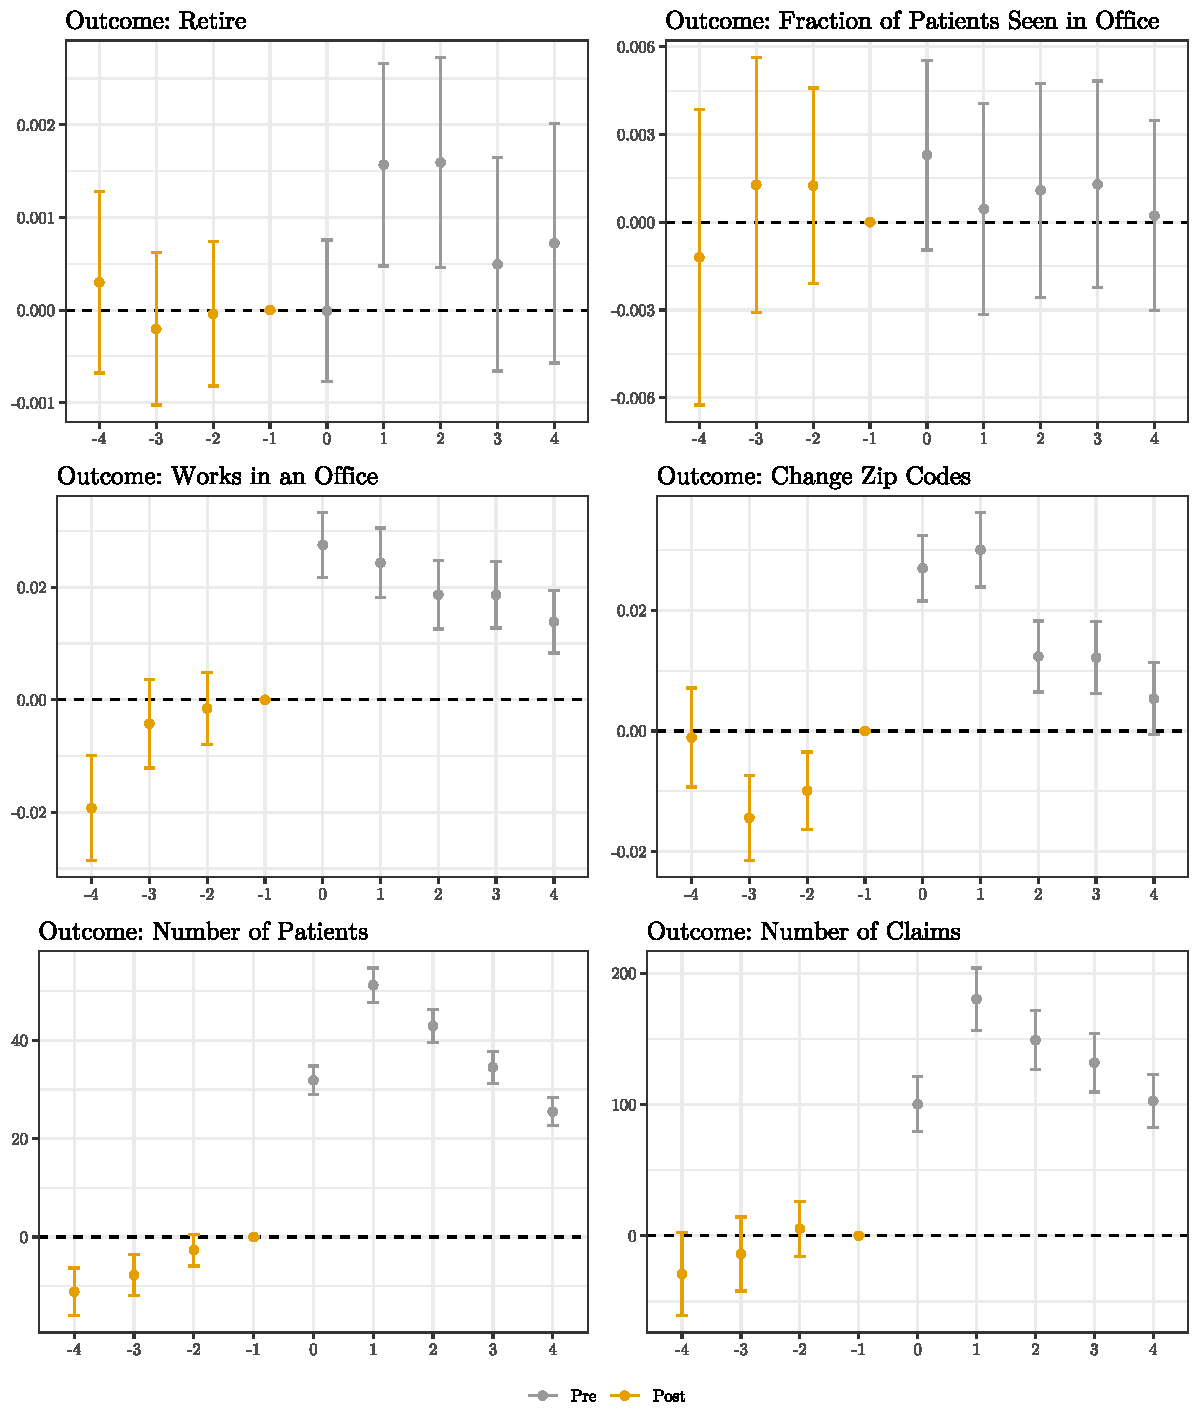
\includegraphics[scale=.8]{Objects/twfe_plot.pdf}
    \label{fig:twfe}
    \vspace{2mm}
    \caption*{\footnotesize{\textit{Notes:} Event study plots from two way fixed effects estimation are shown for each outcome variable.}}
\end{figure}

One method that addresses issues with the TWFE specification by differencing out fixed effects is established in \citeauthor{gardner2021two} (\citeyear{gardner2021two}). This approach is commonly known as two stage difference in differences and is very clever. However, the approach requires a group of never-treated units as the comparison group, a drawback for my study in that I remove all never-treated units to utilize all years of MD-PPAS data, and because never-treated hospitals are likely compositionally different from those treated in the majority of the sample. Nevertheless, I limit the years of data to 2009-2015 and present estimates of this estimator in Figure \ref{fig:estimators}. Generally, the results have the same sign with a slightly larger magnitude, driven by the inclusion of never-treated units. 

\begin{figure}
    \centering
    \caption{Alternative Estimators}
    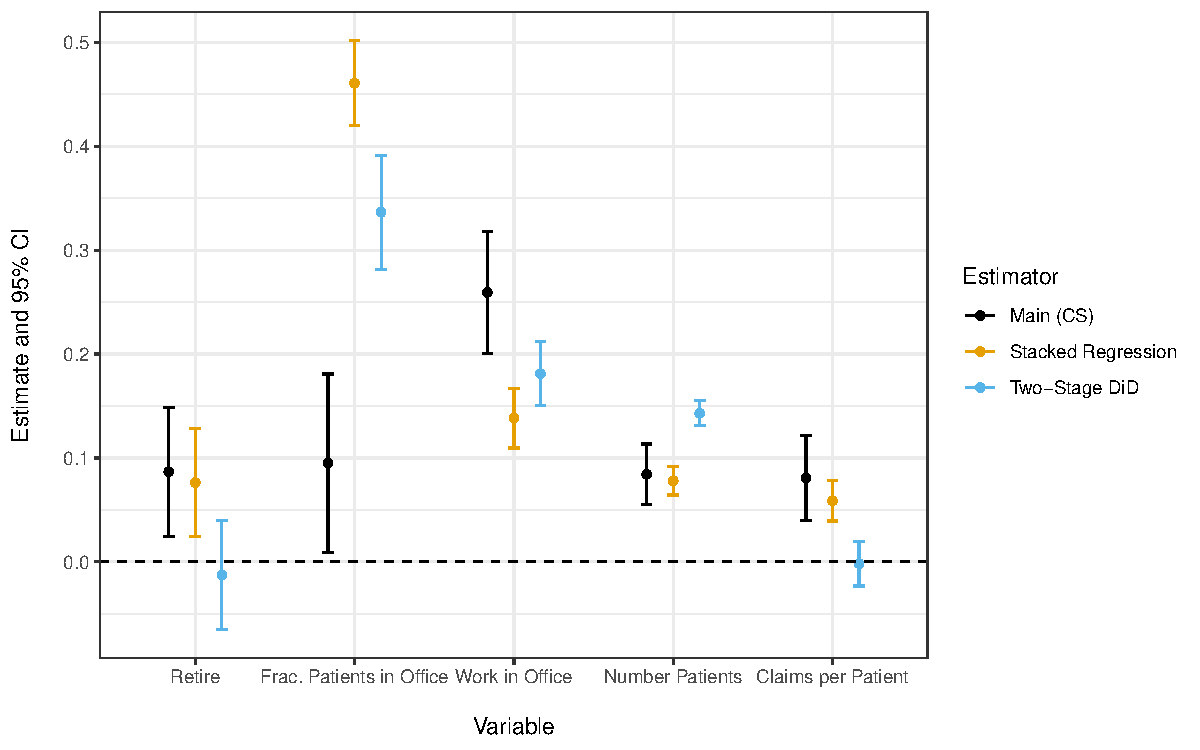
\includegraphics[scale=.7]{Objects/estimators_plot.pdf}
    \label{fig:estimators}
\end{figure}

Another estimation method first used by \citeauthor{cengiz2019effect} (\citeyear{cengiz2019effect}) is commonly known as stacked regression. In this method, one re-frames event study data into groups of sub-experiments that are then stacked on top of each other, defining a group of treated units and ``clean" control units. The drawback of this method is choosing an event study window that must be the same for each treatment group, where a large window eliminates many treated units and a small window does not allow for estimation over many years. I present the results using this method with an event window of one year in Figure \ref{fig:estimators}. The results are very similar to the main specification, with a smaller magnitude in some cases. 





\section{Heterogeneity Analysis}

The main analysis focuses on the differential effects of technology for older vs. younger physicians. However, another important question is whether physicians in rural vs. urban settings respond differently to the technology since the implications for behavior changes are high in areas that already suffer from access to care issues. Thus, I present average treatment effects for each outcome where the sample is split between physicians in rural and urban areas. Further, to investigate the same idea, I present results for physicians who typically work at small hospitals vs. those who typically work at large hospitals. These average treatment effects are shown in Figure \ref{fig:1}. The results do not differ along these dimensions. This is fascinating in that technology is creating these adverse effects across completely different practice environments.


\begin{figure}[t!]
\begin{subfigure}{0.48\textwidth}
\caption{Retire}
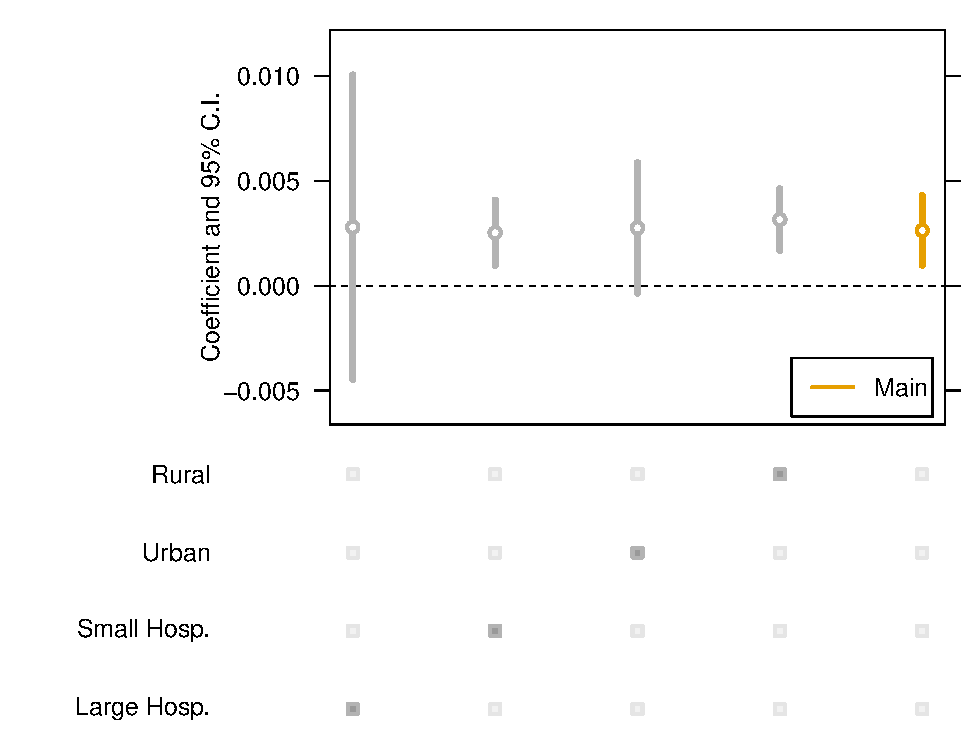
\includegraphics[width=\linewidth]{Objects/retire_heterog.pdf}
\label{fig:a}
\end{subfigure}\hspace*{\fill}
\begin{subfigure}{0.48\textwidth}
\caption{Fraction of Patients in Office}
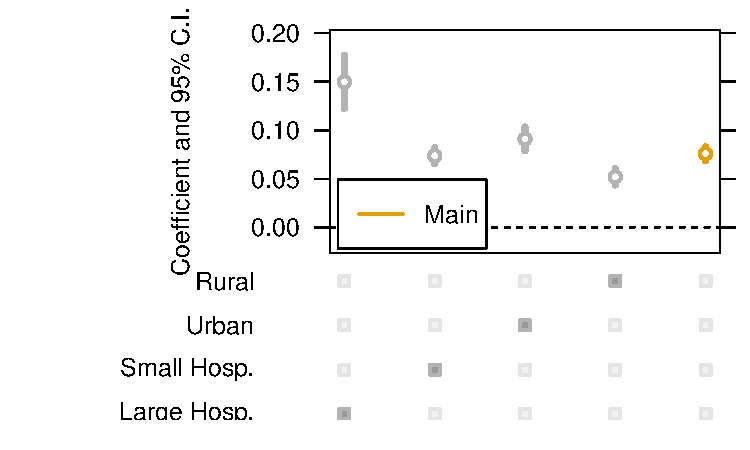
\includegraphics[width=\linewidth]{Objects/office_frac_heterog.pdf}
\label{fig:b}
\end{subfigure}

\medskip
\begin{subfigure}{0.48\textwidth}
\caption{Indicator for Office }
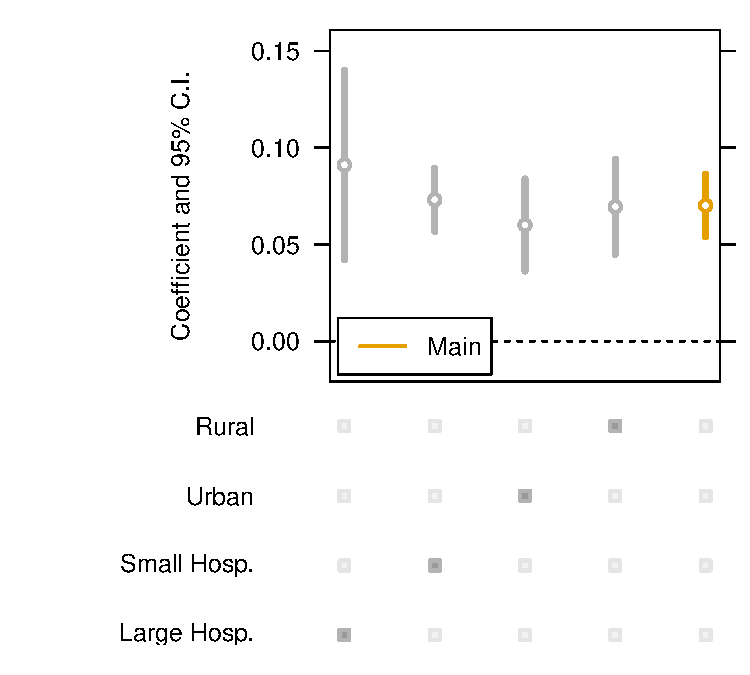
\includegraphics[width=\linewidth]{Objects/office_ind_heterog.pdf}
 \label{fig:c}
\end{subfigure}\hspace*{\fill}
\begin{subfigure}{0.48\textwidth}
\caption{Patient Count} 
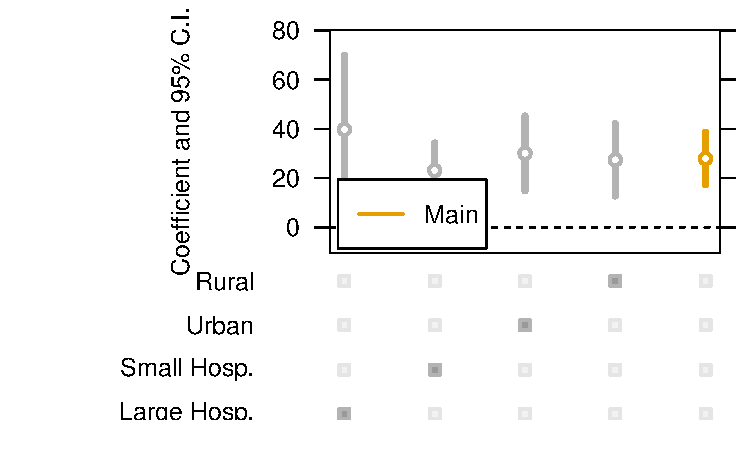
\includegraphics[width=\linewidth]{Objects/patient_heterog.pdf}
\label{fig:d}
\end{subfigure}

\medskip
\begin{subfigure}{0.48\textwidth}
\caption{Claims Per Patient} 
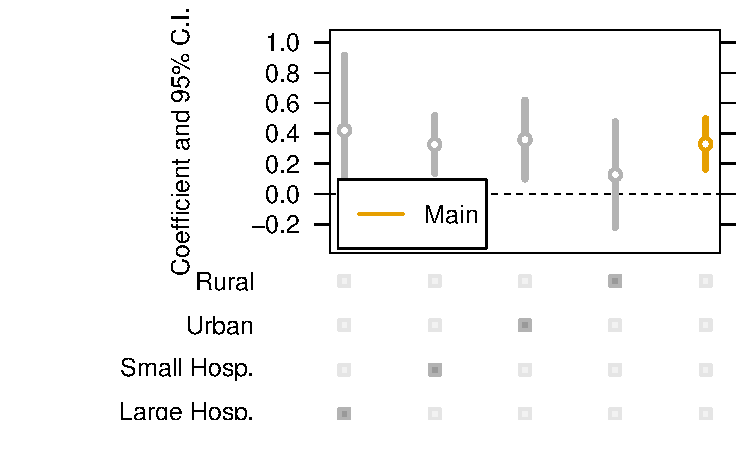
\includegraphics[width=\linewidth]{Objects/claim_per_patient_heterog.pdf}
\label{fig:e}
\end{subfigure}\hspace*{\fill}

\caption{Heterogeneity Analysis} \label{fig:1}
\end{figure}





















\end{document}